\documentclass[main.tex]{subfiles}
\begin{document}

\href{https://www2.seas.gwu.edu/~simhaweb/quantum/modules/module4/module4.html}{Module 4: Quantum Linear Algebra, Part 2}

\subsection{What do we call a group of interacting qubits?}
    Let's first examine the same question for classical bits: In classical logic, multiple bits interact through logic gates. For example reference Figure \ref{fig:01bits}
    
    \begin{figure}
        \centering
        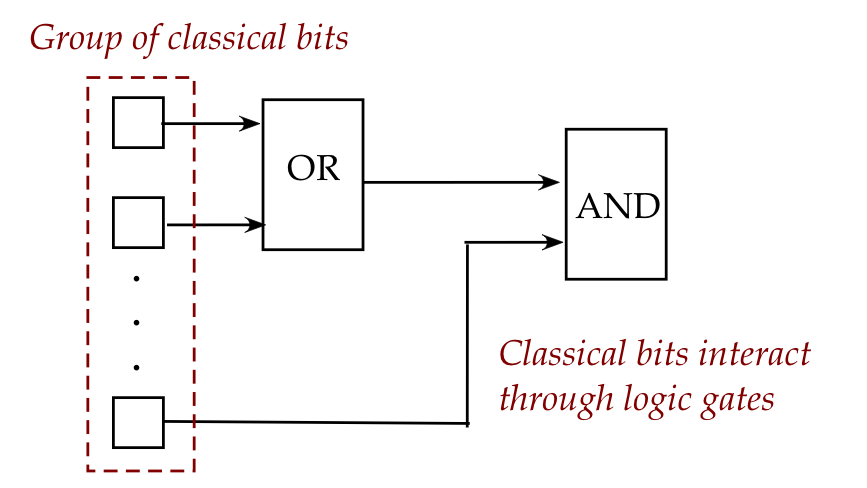
\includegraphics[width=4in]{notes/figs/n06/01bits.png}
        \caption{Classical bits logical gates}
        \label{fig:01bits}
    \end{figure}  
    
    Let's think of the bit as a device that can hold one of the values (states) 0 or $1 .$ At any given moment, a bit can either be in state 0 or in state $1 .$ Interactions are arranged through logic gates. What happens to the outputs? Some of the outputs can come back and be used to replace change the state of a bit. But alternatively, some outputs can be made to change other bits (not pictured). We typically use the term register for a group of classical bits that are primed for interaction. Note: there's no sense in which a group of bits can be considered a "larger bit". Let's now ask the same question about qubits reference Figure \ref{fig:02bits2}.
    
    \begin{figure}
        \centering
        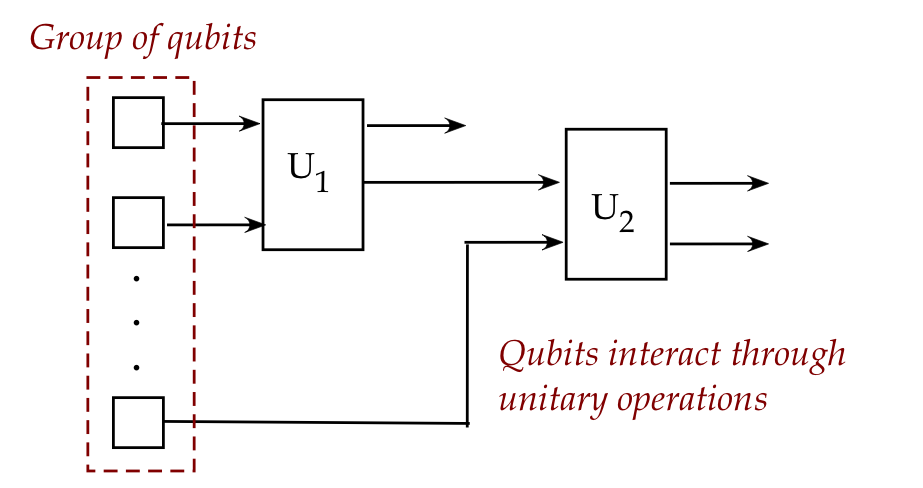
\includegraphics[width=4in]{notes/figs/n06/02bits2.png}
        \caption{Qubit unitary operations}
        \label{fig:02bits2}
    \end{figure} 
    
    Here, the devices are qubits and the values (states) they can hold are complex 2D vectors. At any given moment, a qubit's state can be any valid unit-length 2D vector such as $|\psi\rangle=\alpha|0\rangle+\beta|1\rangle$. Interactions between qubits are arranged through unitary operations that change the qubits directly (as opposed to changing other qubits.) Now for the surprise reference Figure \ref{fig:03bits2b}.
    
    \begin{figure}
        \centering
        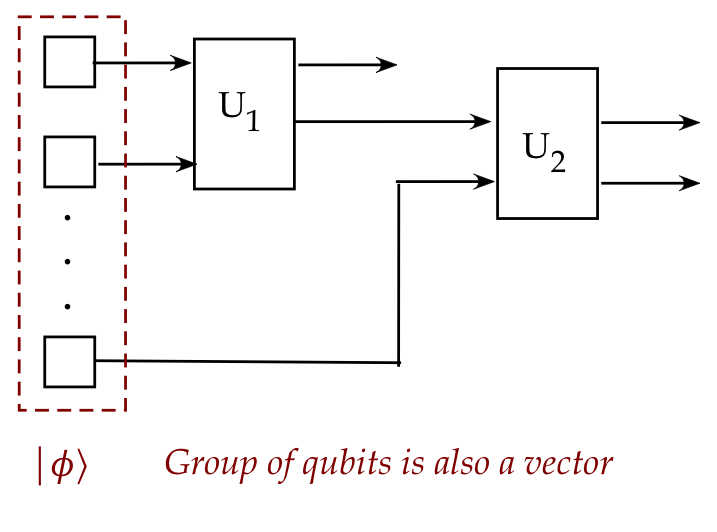
\includegraphics[width=4in]{notes/figs/n06/03bits2b.png}
        \caption{Qubits as a vector}
        \label{fig:03bits2b}
    \end{figure} 
    
    A group of qubits, each a vector, is itself a larger vector. The whole group of qubits can be treated as a single vector with a single combined state. This was not possible with classical bits. Does it matter? It certainly does, in many ways. First, as we will see in this module, the entire theory of linear algebra we developed for single qubits extends to the vectors and unitary operations for multiple qubits. But there are surprising implications to this larger vector for the group of qubits. Suppose we use the standard basis to represent the individual vectors in a three qubit example: One possible set of values is: $|0\rangle,|0\rangle,|0\rangle$. We write the combined vector as $|000\rangle$. Another possible set is: $|1\rangle,|0\rangle,|1\rangle$. The combined vector is $|101\rangle$. In this way, it will turn out that the larger vector space has an 8-vector basis: $|000\rangle,|001\rangle,|010\rangle, \ldots,|110\rangle,|111\rangle$. Now for the first surprising implication: With the three-qubit example, because there are 8 basis vectors, any unit-length linear combination is also a valid state, e.g.
    
    $$
    \frac{1}{\sqrt{8}}(|000\rangle+|001\rangle+\ldots+|111\rangle)
    $$
    
    Thus, with $n$ qubits, any (unit-length) linear combination of $2^{n}$ basis vectors is a potential state. Compare with classical: Classical: $n$ bits can hold one of $2^{n}$ combinations, Each state is an $\mathrm{n}$-bit binary combination. Quantum: $n$ qubits can hold one of an uncountable number linear combinations, Each state is a linear combination of $2^{n}$ basis vectors. Thus, a single quantum state for n-qubits has the potential to be exponentially larger than a single classical state! We will later see that an equal-weight combination of all $2^{n}$ basis vectors is in fact a starting state common to many algorithms.
    Entanglement: the other surprise. Consider a two-qubit system in the state
    
    $$
    |\psi\rangle=\frac{1}{\sqrt{2}}(|01\rangle+|10\rangle)
    $$
    
    (What precisely this means we will see later.) Thus, what we can infer is, when measured in the standard basis: First qubit state $=|0\rangle \Longleftrightarrow|1\rangle=$ second qubit state. First qubit state $=|1\rangle \Longleftrightarrow|0\rangle=$ second qubit state. It can never be that they are both in the same state. What is profoundly interesting (and useful) is that the two qubits above can be physically separated while maintaining this property reference Figure \ref{fig:04bits3}.
    
    \begin{figure}
        \centering
        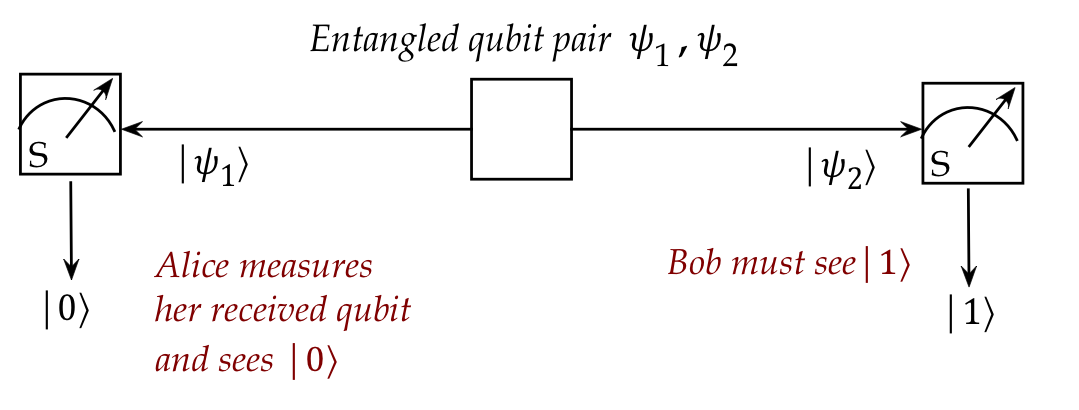
\includegraphics[width=4in]{notes/figs/n06/04bits3.png}
        \caption{Entangled qubit pair}
        \label{fig:04bits3}
    \end{figure} 
    
    Then, if Alice measures the first qubit, the outcome exactly determines what Bob sees with the second qubit. Instantaneously, no matter the distance between Alice and Bob. Indeed, this feature is exploited in communication protocols. Thus, the goal of this module is to develop the theory that connects the larger multi-qubit vector from the individual qubit vectors. For this, we need a new linear algebra construct: the tensor product.

\subsection{Tensor products of vectors}

    A tensor product of two vectors (for the two qubit case) creates a larger vector. Let's use a simple two-qubit example to see what's needed to build this larger vector reference Figure \ref{fig:05tensor1}.

    \begin{figure}
        \centering
        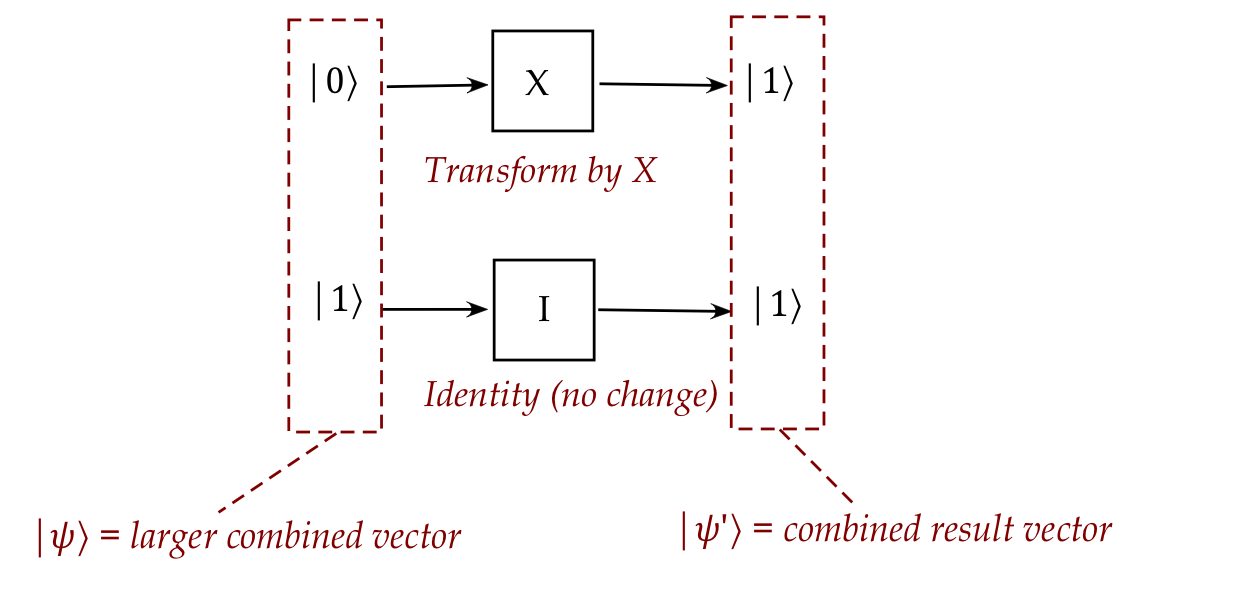
\includegraphics[width=4in]{notes/figs/n06/05tensor1.png}
        \caption{tensor product of two vectors}
        \label{fig:05tensor1}
    \end{figure} 
    
    In this setup: The first qubit is flipped via the $X$ operator. The second qubit remains the same. This is the same as applying the identity operator $I$. Looked at individually, we would write
    
    $$
    \begin{aligned}
    X|0\rangle &=\left[\begin{array}{ll}
    0 & 1 \\
    1 & 0
    \end{array}\right]\left[\begin{array}{l}
    1 \\
    0
    \end{array}\right]=\left[\begin{array}{l}
    0 \\
    1
    \end{array}\right] \\
    I|1\rangle &=\left[\begin{array}{ll}
    1 & 0 \\
    0 & 1
    \end{array}\right]\left[\begin{array}{l}
    0 \\
    1
    \end{array}\right]=\left[\begin{array}{l}
    0 \\
    1
    \end{array}\right]
    \end{aligned}
    $$
    
    Suppose we had A larger vector $|\psi\rangle$ that described the initial combined state of the qubits. A larger vector $\left|\psi^{\prime}\right\rangle$ for the result. A larger unitary operator $U$ to achieve the combined transformation Then, we must have
    
    $$
    U|\psi\rangle=\left|\psi^{\prime}\right\rangle
    $$
    
    As it turns out, this is exactly what will transpire: We will devise special notation to combine vectors and operators: The tensor symbol $\otimes$. For the above example
    
    $$
    U|\psi\rangle=\left[\begin{array}{llll}
    0 & 0 & 1 & 0 \\
    0 & 0 & 0 & 1 \\
    1 & 0 & 0 & 0 \\
    0 & 1 & 0 & 0
    \end{array}\right]\left[\begin{array}{l}
    0 \\
    1 \\
    0 \\
    0
    \end{array}\right]=\left[\begin{array}{l}
    0 \\
    0 \\
    0 \\
    1
    \end{array}\right]=\left|\psi^{\prime}\right\rangle
    $$
    $$
    |\psi\rangle=|0\rangle \otimes|1\rangle=\left[\begin{array}{l}
    0 \\
    1 \\
    0 \\
    0
    \end{array}\right]
    $$
    $$
    \left|\psi^{\prime}\right\rangle=|1\rangle \otimes|1\rangle=\left[\begin{array}{l}
    0 \\
    0 \\
    0 \\
    1
    \end{array}\right]
    $$
    $$
    U=X \otimes I=\left[\begin{array}{llll}
    0 & 0 & 1 & 0 \\
    0 & 0 & 0 & 1 \\
    1 & 0 & 0 & 0 \\
    0 & 1 & 0 & 0
    \end{array}\right]
    $$
    
    Next, let's ask: what kinds of properties are desirable or necessary for tensors? The first property, one that we will impose, is distribution of $\otimes$ over addition: Given individual vectors $\left|v_{1}\right\rangle,\left|v_{2}\right\rangle,|w\rangle$ the following needs to be true:
    
    $$
    \left(\left|v_{1}\right\rangle+\left|v_{2}\right\rangle\right) \otimes|w\rangle=\left(\left|v_{1}\right\rangle \otimes|w\rangle\right)+\left(\left|v_{2}\right\rangle \otimes|w\rangle\right)
    $$
    
    And symmetrically
   
    $$
    |w\rangle \otimes\left(\left|v_{1}\right\rangle+\left|v_{2}\right\rangle\right)=\left(|w\rangle \otimes\left|v_{1}\right\rangle\right)+\left(|w\rangle \otimes\left|v_{2}\right\rangle\right)
    $$
    
    Such a property is verifiable experimentally. Once we accept distribution, we see that
    
    $$
    2|v\rangle \otimes|w\rangle=(|v\rangle+|v\rangle) \otimes|w\rangle=(|v\rangle \otimes|w\rangle)+(|v\rangle \otimes|w\rangle)=2(|v\rangle \otimes|w\rangle)
    $$
    
    In general, this would also mean
    
    $$
    (k|v\rangle) \otimes|w\rangle=k(|v\rangle \otimes|w\rangle)=(|v\rangle \otimes k|w\rangle
    $$
    
    for any integer $k$. It would have to be a very strange operation to only work for integers, so in general:
    
    $$
    (\alpha|v\rangle) \otimes|w\rangle=\alpha(|v\rangle \otimes|w\rangle)=(|v\rangle \otimes \alpha|w\rangle
    $$
    
    for any complex number $\alpha$. With these requirements on $\otimes$ we are almost safely in the comfort zone of traditional linearity:
    
    $$
    \begin{aligned}
    &\left(\alpha\left|v_{1}\right\rangle+\beta\left|v_{2}\right\rangle\right) \otimes|w\rangle=\alpha\left(\left|v_{1}\right\rangle \otimes|w\rangle\right)+\beta\left(\left|v_{2}\right\rangle \otimes|w\rangle\right) \\
    &\left(|w\rangle \otimes \alpha\left|v_{1}\right\rangle+\beta\left|v_{2}\right\rangle\right)=\alpha\left(|w\rangle \otimes\left|v_{1}\right\rangle\right)+\beta\left(|w\rangle \otimes\left|v_{2}\right\rangle\right)
    \end{aligned}
    $$
    
    Why did we say almost? Recall from above:
    
    $$
    \alpha(|v\rangle \otimes|w\rangle)=(\alpha|v\rangle) \otimes|w\rangle=(|v\rangle \otimes \alpha|w\rangle) \neq(\alpha|v\rangle \otimes \alpha|w\rangle)
    $$
    
    That is, the scalar $\alpha$ when pushed inside the tensor product attaches to only one of the operands. Either the left operand or the right, but not both. In fact
    
    $$
    (\alpha|v\rangle \otimes \alpha|w\rangle)=\alpha^{2}(|v\rangle \otimes|w\rangle)
    $$
    
    We can then push two scalars differently, as in:
    
    $$
    \alpha \beta(|v\rangle \otimes|w\rangle)=\alpha|v\rangle \otimes \beta|w\rangle
    $$
    
    This property is called bilinearity. This is going to be most useful when we combine operators as in:
    
    $$
    (X \otimes I)(|0\rangle \otimes|1\rangle)=(X|0\rangle \otimes I|1\rangle)=(|1\rangle \otimes|1\rangle)
    $$
    
    More about this in the next section. Next, with 2-qubit examples, let's now figure out how to build the larger vectors: We know that a single-qubit vector has two coordinates because it's a 2D vector, as in:
    
    $$
    |1\rangle=\left[\begin{array}{l}
    0 \\
    1
    \end{array}\right]
    $$
    
    Thus, when we combine two such vectors (one per qubit), we'll have four numbers That is, a 4-component vector. The standard basis for 4-component vectors is:
    
    $$
    \left[\begin{array}{l}
    1 \\
    0 \\
    0 \\
    0
    \end{array}\right] \quad\left[\begin{array}{l}
    0 \\
    1 \\
    0 \\
    0
    \end{array}\right] \quad\left[\begin{array}{l}
    0 \\
    0 \\
    1 \\
    0
    \end{array}\right] \quad\left[\begin{array}{l}
    0 \\
    0 \\
    0 \\
    1
    \end{array}\right]
    $$
    
    Now, the basis vectors for each individual qubit are
    
    $$
    \left[\begin{array}{l}
    1 \\
    0
    \end{array}\right] \quad\left[\begin{array}{l}
    0 \\
    1
    \end{array}\right]
    $$
    
    So, somehow the four possible combinations of these need to produce the four larger basis vectors:
    
    $$
    \left[\begin{array}{l}
    1 \\
    0
    \end{array}\right] \otimes\left[\begin{array}{l}
    1 \\
    0
    \end{array}\right]=\left[\begin{array}{l}
    1 \\
    0 \\
    0 \\
    0
    \end{array}\right] \quad\left[\begin{array}{l}
    1 \\
    0
    \end{array}\right] \otimes\left[\begin{array}{l}
    0 \\
    1
    \end{array}\right]=\left[\begin{array}{l}
    0 \\
    1 \\
    0 \\
    0
    \end{array}\right] \quad\left[\begin{array}{l}
    0 \\
    1
    \end{array}\right] \otimes\left[\begin{array}{l}
    1 \\
    0
    \end{array}\right]=\left[\begin{array}{l}
    0 \\
    0 \\
    1 \\
    0
    \end{array}\right] \quad\left[\begin{array}{l}
    0 \\
    1
    \end{array}\right] \otimes\left[\begin{array}{l}
    0 \\
    1
    \end{array}\right]=\left[\begin{array}{l}
    0 \\
    0 \\
    0 \\
    1
    \end{array}\right]
    $$
    
    That is we need to figure out: what rule takes two smaller vectors to produce the larger? The answer comes from bilinearity: Let's look at
    
    $$
    \left[\begin{array}{c}
    \alpha_{1} \\
    0
    \end{array}\right] \otimes\left[\begin{array}{c}
    \beta_{1} \\
    0
    \end{array}\right]=\alpha_{1}\left[\begin{array}{l}
    1 \\
    0
    \end{array}\right] \otimes \beta_{1}\left[\begin{array}{l}
    1 \\
    0
    \end{array}\right]=\alpha_{1} \beta_{1}\left[\begin{array}{l}
    1 \\
    0 \\
    0 \\
    0
    \end{array}\right]=\left[\begin{array}{c}
    \alpha_{1} \beta_{1} \\
    0 \\
    0 \\
    0
    \end{array}\right]
    $$
    
    And
    
    $$
    \left[\begin{array}{c}
    \alpha_{1} \\
    0
    \end{array}\right] \otimes\left[\begin{array}{c}
    0 \\
    \beta_{2}
    \end{array}\right]=\alpha_{1}\left[\begin{array}{l}
    1 \\
    0
    \end{array}\right] \otimes \beta_{2}\left[\begin{array}{l}
    0 \\
    1
    \end{array}\right]=\alpha_{1} \beta_{2}\left[\begin{array}{l}
    0 \\
    1 \\
    0 \\
    0
    \end{array}\right]=\left[\begin{array}{c}
    0 \\
    \alpha_{1} \beta_{2} \\
    0 \\
    0
    \end{array}\right]
    $$
    
    where we're naming the constants in a certain way to clarify what comes next. Let's do the remaining two:
    
    $$
    \left[\begin{array}{c}
    0 \\
    \alpha_{2}
    \end{array}\right] \otimes\left[\begin{array}{c}
    \beta_{1} \\
    0
    \end{array}\right]=\alpha_{2}\left[\begin{array}{l}
    0 \\
    1
    \end{array}\right] \otimes \beta_{1}\left[\begin{array}{l}
    1 \\
    0
    \end{array}\right]=\alpha_{2} \beta_{1}\left[\begin{array}{l}
    0 \\
    0 \\
    1 \\
    0
    \end{array}\right]=\left[\begin{array}{c}
    0 \\
    0 \\
    \alpha_{2} \beta_{1} \\
    0
    \end{array}\right]
    $$
    
    and
    
    $$
    \left[\begin{array}{c}
    0 \\
    \alpha_{2}
    \end{array}\right] \otimes\left[\begin{array}{c}
    0 \\
    \beta_{2}
    \end{array}\right]=\alpha_{2}\left[\begin{array}{l}
    0 \\
    1
    \end{array}\right] \otimes \beta_{2}\left[\begin{array}{l}
    0 \\
    1
    \end{array}\right]=\alpha_{2} \beta_{2}\left[\begin{array}{l}
    0 \\
    0 \\
    0 \\
    1
    \end{array}\right]=\left[\begin{array}{c}
    0 \\
    0 \\
    0 \\
    \alpha_{2} \beta_{2}
    \end{array}\right]
    $$
    
    Adding on both sides gives us
    
    $$
    \left[\begin{array}{l}
    \alpha_{1} \\
    \alpha_{2}
    \end{array}\right] \otimes\left[\begin{array}{l}
    \beta_{1} \\
    \beta_{2}
    \end{array}\right]=\left[\begin{array}{l}
    \alpha_{1} \beta_{1} \\
    \alpha_{1} \beta_{2} \\
    \alpha_{2} \beta_{1} \\
    \alpha_{2} \beta_{2}
    \end{array}\right]
    $$
    
    which, for insight, we can also write as:
    
    $$
    \left[\begin{array}{l}
    \alpha_{1} \\
    \alpha_{2}
    \end{array}\right] \otimes\left[\begin{array}{l}
    \beta_{1} \\
    \beta_{2}
    \end{array}\right]=\left[\begin{array}{c}
    \alpha_{1}\left[\begin{array}{l}
    \beta_{1} \\
    \beta_{2}
    \end{array}\right] \\
    \alpha_{2}\left[\begin{array}{l}
    \beta_{1} \\
    \beta_{2}
    \end{array}\right]
    \end{array}\right]
    $$
    
    Thus, each element of the first vector multiplies into the entire other vector, and all these are stacked up. We now have our rule for computing $|v\rangle \otimes|w\rangle$ for any two $2 \mathrm{D}$ vectors $|v\rangle$ and $|w\rangle$. The same idea can be generalized to n dimensions:

    $$
    \left[\begin{array}{c}
    \alpha_{1} \\
    \vdots \\
    \alpha_{n}
    \end{array}\right] \otimes\left[\begin{array}{c}
    \beta_{1} \\
    \vdots \\
    \beta_{n}
    \end{array}\right]
    =\left[\begin{array}{c}
    \alpha_{1}\left[\begin{array}{c}
    \beta_{1} \\
    \vdots \\
    \beta_{n}
    \end{array}\right] \\
    \alpha_{2}\left[\begin{array}{c}
    \beta_{1} \\
    \vdots \\
    \beta_{n}
    \end{array}\right] \\
    \vdots \\
    \alpha_{n}\left[\begin{array}{c}
    \beta_{1} \\
    \vdots \\
    \beta_{n}
    \end{array}\right]
    \end{array}\right]=\left[\begin{array}{c}
    \alpha_{1} \beta_{1} \\
    \vdots \\
    \alpha_{1} \beta_{n} \\
    \alpha_{2} \beta_{1} \\
    \vdots \\
    \alpha_{2} \beta_{n} \\
    \vdots \\
    \alpha_{n} \beta_{1} \\
    \vdots \\
    \alpha_{n} \beta_{n}
    \end{array}\right]
    $$
    
    This is called the vector tensor product. Note: none of the number-products involve conjugation.
    
    Inner product: Now that we've defined the tensor product to be a vector, that larger vector will have an inner product. For example: Suppose
    
    $$
    |\psi\rangle=|v\rangle \otimes|w\rangle
    $$
    
    is one tensored vector. And let
    
    $$
    |\phi\rangle=|x\rangle \otimes|y\rangle
    $$
    
    be another. Clearly, since $|\psi\rangle$ and $|\phi\rangle$ are vectors, we can compute the inner product
    $\langle\psi \mid \phi\rangle$. Now, in the example above, one can compute inner products of the small vectors $|v\rangle,|w\rangle,|x\rangle,|y\rangle$ in various combinations. Thus, the key question is: can we relate $\langle\psi \mid \phi\rangle$ to the inner products of the smaller vectors? The answer is: yes
    
    $$
    \langle\psi \mid \phi\rangle=\langle\mid v\rangle \otimes|w\rangle|| x\rangle \otimes|y\rangle\rangle=(\langle v \mid x\rangle)(\langle w \mid y\rangle)
    $$
    
    To get some insight into why, let's examine
    
    $$
    \begin{aligned}
    \left.\left.\left\langle\alpha_{1} \mid 0\right\rangle \otimes \beta_{1}|0\rangle\left|\gamma_{1}\right| 0\right\rangle \otimes \delta_{1}|0\rangle\right\rangle &=\left(\left[\begin{array}{c}
    \alpha_{1} \\
    0
    \end{array}\right] \otimes\left[\begin{array}{c}
    \beta_{1} \\
    0
    \end{array}\right]\right)^{\dagger}\left(\left[\begin{array}{c}
    \gamma_{1} \\
    0
    \end{array}\right] \otimes\left[\begin{array}{c}
    \delta_{1} \\
    0
    \end{array}\right]\right) \\
    &=\left(\left[\begin{array}{c}
    \alpha_{1} \beta_{1} \\
    0 \\
    0 \\
    0
    \end{array}\right]\right)\left(\left[\begin{array}{c}
    \gamma_{1} \delta_{1} \\
    0 \\
    0 \\
    0
    \end{array}\right]\right) \\
    &=\alpha_{1}^{*} \beta_{1}^{*} \gamma_{1} \delta_{1}
    \end{aligned}
    $$
    
    Now we can write the latter as
    
    $$
    \left(\alpha_{1}^{*} \gamma_{1}\right)\left(\beta_{1}^{*} \delta_{1}\right)
    $$
    
    This is the direct number-product of the two smaller inner products:
    
    $$
    \left(\alpha_{1}^{*} \gamma_{1}\right)\left(\beta_{1}^{*} \delta_{1}\right)=\left(\left[\begin{array}{c}
    \alpha_{1} \\
    0
    \end{array}\right]^{\dagger}\left[\begin{array}{c}
    \gamma_{1} \\
    0
    \end{array}\right]\right)\left(\left[\begin{array}{c}
    \beta_{1} \\
    0
    \end{array}\right]^{\dagger}\left[\begin{array}{c}
    \delta_{1} \\
    0
    \end{array}\right]\right)=(\langle v \mid x\rangle)(\langle w \mid y\rangle)
    $$
    
    In this way, one can work out the inner product for any linear combination of the basis vectors the inner product. One minor point about convention: When we re-grouped
    
    $$
    \alpha_{1}^{*} \beta_{1}^{*} \gamma_{1} \delta_{1}=\left(\alpha_{1}^{*} \gamma_{1}\right)\left(\beta_{1}^{*} \delta_{1}\right)
    $$
    
    we could have alternatively re-grouped as
    
    $$
    \alpha_{1}^{*} \beta_{1}^{*} \gamma_{1} \delta_{1}=\left(\alpha_{1}^{*} \delta_{1}\right)\left(\beta_{1}^{*} \gamma_{1}\right)
    $$
    
    and defined a different type of inner product. But this would deviate from the left-to-right order we have been using so far. Hence the convention is to define the larger inner product as
    
    $$
    \langle\mid v\rangle \otimes|w\rangle|| x\rangle \otimes|y\rangle\rangle=(\langle v \mid x\rangle)(\langle w \mid y\rangle)
    $$
    
    We will also write the larger inner product as
    
    $$
    \langle\langle v|\otimes\langle w|| \mid x\rangle \otimes| y\rangle\rangle
    $$
    
    where the context makes it clear that the left side in an inner product is row-conjugated.

\subsection{Tensor products of operators}

    Let's turn to building larger, tensored matrices from smaller ones: Let's first describe what we seek: Suppose we have a tensor product like $|v\rangle \otimes|w\rangle$. And suppose we have unitary operators acting on each qubit, as in $A|v\rangle \otimes B|w\rangle$. This will result in a larger vector. What we want is to figure out the larger matrix $C$ such that
    
    $$
    C(|v\rangle \otimes|w\rangle)=A|v\rangle \otimes B|w\rangle
    $$
    
    What we really need is the relationship between $C$ and $A$ and $B$. The relationship is obtained readily through a bit of painstaking multiplication. Let's start with the smaller products: Suppose
    
    $$
    |v\rangle=\left[\begin{array}{l}
    v_{1} \\
    v_{2}
    \end{array}\right] \quad|w\rangle=\left[\begin{array}{l}
    w_{1} \\
    w_{2}
    \end{array}\right]
    $$
    
    and
    
    $$
    A=\left[\begin{array}{ll}
    a_{11} & a_{12} \\
    a_{21} & a_{22}
    \end{array}\right] \quad B=\left[\begin{array}{ll}
    b_{11} & b_{12} \\
    b_{21} & b_{22}
    \end{array}\right]
    $$
    
    Note: the indices 1 and 2 in $v_{1}, v_{2}$ range over the elements (coordinates) inside vectors. Then
    
    $$
    A|v\rangle \otimes B|w\rangle=\left[\begin{array}{l}
    a_{11} v_{1}+a_{12} v_{2} \\
    a_{21} v_{1}+a_{22} v_{2}
    \end{array}\right] \otimes\left[\begin{array}{l}
    b_{11} w_{1}+b_{12} w_{2} \\
    b_{21} w_{1}+b_{22} w_{2}
    \end{array}\right]
    $$
    
    $$
    =\left[\begin{array}{l}
    \left(a_{11} v_{1}+a_{12} v_{2}\right)\left[\begin{array}{l}
    b_{11} w_{1}+b_{12} w_{2} \\
    b_{21} w_{1}+b_{22} w_{2}
    \end{array}\right] \\
    \left(a_{21} v_{1}+a_{22} v_{2}\right)\left[\begin{array}{l}
    b_{11} w_{1}+b_{12} w_{2} \\
    b_{21} w_{1}+b_{22} w_{2}
    \end{array}\right]
    \end{array}\right]
    $$
    
    $=\ldots$ 
    
    a few steps ...
    
    $=\left[\begin{array}{ll}a_{11}\left[\begin{array}{ll}b_{11} & b_{12} \\ b_{21} & b_{22}\end{array}\right] & a_{12}\left[\begin{array}{ll}b_{11} & b_{12} \\ b_{21} & b_{22}\end{array}\right] \\ a_{21}\left[\begin{array}{ll}b_{11} & b_{12} \\ b_{21} & b_{22}\end{array}\right] & a_{22}\left[\begin{array}{ll}b_{11} & b_{12} \\ b_{21} & b_{22}\end{array}\right]\end{array}\right]\left[\begin{array}{l}v_{1} w_{1} \\ v_{1} w_{2} \\ v_{2} w_{1} \\ v_{2} w_{2}\end{array}\right]$ $=\left[\begin{array}{ll}a_{11}\left[\begin{array}{ll}b_{11} & b_{12} \\ b_{21} & b_{22}\end{array}\right] & a_{12}\left[\begin{array}{ll}b_{11} & b_{12} \\ b_{21} & b_{22}\end{array}\right] \\ a_{21}\left[\begin{array}{ll}b_{11} & b_{12} \\ b_{21} & b_{22}\end{array}\right] & a_{22}\left[\begin{array}{ll}b_{11} & b_{12} \\ b_{21} & b_{22}\end{array}\right]\end{array}\right]|v\rangle \otimes|w\rangle$
    
    - Thus,
    
    $$
    C=\left[\begin{array}{ll}
    a_{11}\left[\begin{array}{ll}
    b_{11} & b_{12} \\
    b_{21} & b_{22}
    \end{array}\right] & a_{12}\left[\begin{array}{ll}
    b_{11} & b_{12} \\
    b_{21} & b_{22}
    \end{array}\right] \\
    a_{21}\left[\begin{array}{ll}
    b_{11} & b_{12} \\
    b_{21} & b_{22}
    \end{array}\right] & a_{22}\left[\begin{array}{ll}
    b_{11} & b_{12} \\
    b_{21} & b_{22}
    \end{array}\right]
    \end{array}\right]
    $$
    
    We now have a way to tensor matrices. We will use the same notation as we did with vectors and define
    
    $$
    C=A \otimes B
    $$
    
    Notice that, with this definition,
    
    $$
    (A \otimes B)(|v\rangle \otimes|w\rangle)=(A|v\rangle \otimes B|w\rangle)
    $$
    
    Which is a form of bilinearity for operators. The same idea generalizes to $\mathrm{n}$ dimensions. Summary so far: We have seen how two vectors representing two qubits can be combined into a single vector for both referenced in Figure \ref{fig:06tensor1}.
    
    \begin{figure}
        \centering
        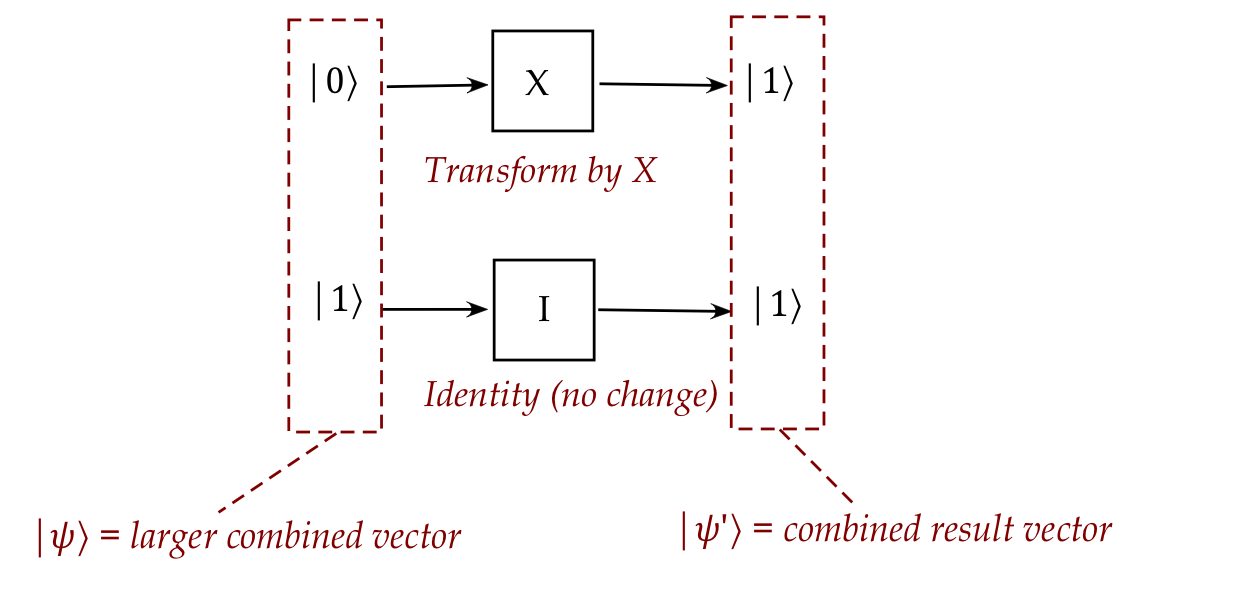
\includegraphics[width=4in]{notes/figs/n06/06tensor1.png}
        \caption{vector combination}
        \label{fig:06tensor1}
    \end{figure} 
    
    We've also seen how to combine unitary operators. What we'd like is to extend the theory so that: It naturally handles $n$ qubits through the same tensor product, as in:
    
    $$
    |v\rangle=\left|v_{1}\right\rangle \otimes \ldots \otimes\left|v_{n}\right\rangle
    $$
    
    Projectors and Hermitians are also combinable with tensors, and maintain their properties. The combining and tensoring is flexible enough to allow various combinations of bits to be operated on: For example: if we only wanted to apply an operator to qubits 1 and 3, but not 2. We'll proceed in four parts: 1. Understanding the vector space that results from multiple qubits. 2. Building larger projectors from smaller ones. 3. Building larger Hermitians from smaller ones. 4. Showing that unitary properties hold with the operator tensor.

\subsection{Relationship between the smaller and larger bases}

    Recall the tensor product of two vectors, which incidentally can be from different-dimensional spaces: Suppose $|v\rangle=\left(\alpha_{1}, \ldots, \alpha_{m}\right)$ and $|w\rangle=\left(\beta_{1}, \ldots, \beta_{n}\right)$ Then
    
    $$
    |v\rangle \otimes|w\rangle=\left[\begin{array}{r}
    \alpha_{1} \\
    \vdots \\
    \alpha_{m}
    \end{array}\right] \otimes\left[\begin{array}{r}
    \beta_{1} \\
    \vdots \\
    \beta_{n}
    \end{array}\right]
    =\left[\begin{array}{c}
    \alpha_{1}\left[\begin{array}{c}
    \beta_{1} \\
    \vdots \\
    \beta_{n}
    \end{array}\right] \\
    \alpha_{2}\left[\begin{array}{c}
    \beta_{1} \\
    \vdots \\
    \beta_{n}
    \end{array}\right] \\
    \vdots \\
    \alpha_{m}\left[\begin{array}{c}
    \beta_{1} \\
    \vdots \\
    \beta_{n}
    \end{array}\right]
    \end{array}\right]=\left[\begin{array}{c}
    \alpha_{1} \beta_{1} \\
    \vdots \\
    \alpha_{1} \beta_{n} \\
    \alpha_{2} \beta_{1} \\
    \vdots \\
    \alpha_{2} \beta_{n} \\
    \vdots \\
    \alpha_{m} \beta_{1} \\
    \vdots \\
    \alpha_{m} \beta_{n}
    \end{array}\right]
    $$
    
    For example, with two qubits, $m=n=2$ Consider the two qubit case: Let $|v\rangle,\left|v^{\perp}\right\rangle$ be basis vectors for one qubit. $|w\rangle,\left|w^{\perp}\right\rangle$ be basis vectors for the other. We know that the inner product of the tensored vectors
    
    $$
    \left.\left.\langle\mid v\rangle \otimes|w\rangle|| v^{\perp}\right\rangle \otimes\left|w^{\perp}\right\rangle\right\rangle=\left\langle v \mid v^{\perp}\right\rangle\left\langle w \mid w^{\perp}\right\rangle=0
    $$
    
    That is, the vectors $|v\rangle \otimes|w\rangle$ and $\left|v^{\perp}\right\rangle \otimes\left|w^{\perp}\right\rangle$ are orthogonal. At the same time, for example
    
    $$
    \left.\left.\langle\mid v\rangle \otimes\left|w^{\perp}\right\rangle|| v\right\rangle \otimes\left|w^{\perp}\right\rangle\right\rangle=\langle v \mid v\rangle\left\langle w^{\perp} \mid w^{\perp}\right\rangle=1
    $$
    
    In this way, one can check that every pairing of smaller basis vectors, one from each qubit results in:
    
    $|v\rangle \otimes|w\rangle$, $|v\rangle \otimes\left|w^{\perp}\right\rangle \quad\left|v^{\perp}\right\rangle \otimes|w\rangle \quad\left|v^{\perp}\right\rangle \otimes\left|w^{\perp}\right\rangle$ These are unit-length and mutually orthogonal. One could ask: are these larger vectors a basis for some space? They indeed are. Suppose $|v\rangle,\left|v^{\perp}\right\rangle$ are basis vectors for vector space $V$. And $|w\rangle,\left|w^{\perp}\right\rangle$ are basis vectors for vector space $W$. Then, the four tensored vectors above are basis vectors for a space we will call $V \otimes W$. This space $V \otimes W$ is the span of those vectors:
    
    $$
    V \otimes W=\operatorname{span}\left\{|v\rangle \otimes|w\rangle,|v\rangle \otimes\left|w^{\perp}\right\rangle,\left|v^{\perp}\right\rangle \otimes|w\rangle,\left|v^{\perp}\right\rangle \otimes\left|w^{\perp}\right\rangle\right\}
    $$
    
    Now let's generalize to $n$ qubits: Let $B_{i}=\left\{\left|v_{i}\right\rangle,\left|v_{i}^{\perp}\right\rangle\right\}$ be the set of basis vectors for the i-th qubit's vector space $V_{i}$. Note: the indices now label vectors not their components. Then the space $V=V_{1} \otimes \ldots \otimes V_{n}$ has the $2^{n}$ vectors $\left|x_{1}\right\rangle \otimes \ldots \otimes\left|x_{n}\right\rangle$ where each $\left|x_{i}\right\rangle \in B_{i}$. That is, pick one of the two vectors in each basis. There are $2^{n}$ such choices.Each such choice is a one basis vector for $V=V_{1} \otimes \ldots \otimes V_{n}$. Example with 3 qubits and standard basis: Each qubit has basis $|0\rangle,|1\rangle$. The $2^{3}$ possible combinations are
    
    \begin{align*}
    |0\rangle \otimes|0\rangle \otimes|0\rangle & =|000\rangle\\
    |0\rangle \otimes|0\rangle \otimes|1\rangle & =|001\rangle\\
    |0\rangle \otimes|1\rangle \otimes|0\rangle & =|010\rangle\\
    |0\rangle \otimes|1\rangle \otimes|1\rangle & =|011\rangle\\
    |1\rangle \otimes|0\rangle \otimes|0\rangle & =|100\rangle\\
    |1\rangle \otimes|0\rangle \otimes|1\rangle & =|101\rangle\\
    |1\rangle \otimes|1\rangle \otimes|0\rangle & =|110\rangle\\
    |1\rangle \otimes|1\rangle \otimes|1\rangle & =|111\rangle\\
    |1\rangle \otimes|1\rangle \otimes|1\rangle & =|111\rangle
    \end{align*}
    
    On the right side, we're introducing a shorthand notation (more about this later). For 2 qubits in the standard basis:
    
    \begin{align*}
        |0\rangle \otimes|0\rangle & =|00\rangle\\
        |0\rangle \otimes|1\rangle & =|01\rangle\\
        |1\rangle \otimes|0\rangle & =|10\rangle\\
        |1\rangle \otimes|1\rangle & =|11\rangle
    \end{align*}

    This raises an interesting question: Consider the 2-qubit case. We can construct a larger vector in two different ways. One way: tensor two vectors, one from each space:
    $|v\rangle \otimes|w\rangle=(\alpha|0\rangle+\beta|1\rangle) \otimes(\gamma|0\rangle+\delta|1\rangle)$
    For example:
    
    $$
    \begin{aligned}
    &\left(\frac{1}{\sqrt{2}}|0\rangle+\frac{1}{\sqrt{2}}|1\rangle\right) \otimes\left(\frac{1}{\sqrt{2}}|0\rangle+\frac{1}{\sqrt{2}}|1\rangle\right) \\
    =& \frac{1}{2}(|0\rangle \otimes|0\rangle)+\frac{1}{2}(|0\rangle \otimes|1\rangle)+\frac{1}{2}(|1\rangle \otimes|0\rangle)+\frac{1}{2}(|1\rangle \otimes|1\rangle) \\
    =& \frac{1}{2}(|00\rangle+|01\rangle+|10\rangle+|11\rangle)
    \end{aligned}
    $$
    
    where the last part uses the shorter notation. The other way: use the basis of the larger space and build a linear combination in the larger space: 
    
    $$
    \begin{aligned}
    & a_{00}(|0\rangle \otimes|0\rangle)+a_{01}(|0\rangle \otimes|1\rangle)+a_{10}(|1\rangle \otimes|0\rangle)+a_{11}(|1\rangle \otimes|1\rangle) \\
    =& a_{00}|00\rangle+a_{01}|01\rangle+a_{10}|10\rangle+a_{11}|11\rangle
    \end{aligned}
    $$
    
    where $a_{00}, a_{01}, a_{10}, a_{11}$ are any complex numbers so that the vector above is unit-length, i.e.,
    
    $$
    \left|a_{00}\right|^{2}+\left|a_{01}\right|^{2}+\left|a_{10}\right|^{2}+\left|a_{11}\right|^{2}=1
    $$
    
    For example:
    
    $$
    0|00\rangle+\frac{1}{\sqrt{2}}|01\rangle+\frac{1}{\sqrt{2}}|10\rangle+0|11\rangle=\frac{1}{\sqrt{2}}(|01\rangle+|10\rangle)
    $$
    
    Here: $a_{00}=a_{11}=0, a_{01}=a_{10}=\frac{1}{\sqrt{2}}$ The question then is: are the two different ways equivalent? The answer: no. And with important implications, as we'll see.

\subsection{Useful properties of tensors}

    We'll now list and prove a number of properties that will serve as the foundation for the multi-qubit setting: Proposition 4.1: Tensoring preserves unit length. Proof: As a result of the inner product $\langle\langle v|\otimes\langle w|| \mid v\rangle \otimes| w\rangle\rangle=\langle v \mid v\rangle\langle w \mid w\rangle=1$ when $|v\rangle,|w\rangle$ are unit-length. Application: We do not need to worry about normalizing when tensoring. Proposition 4.2: If $A, B, C, D$ are operators then $(A \otimes B)(C \otimes D)=A C \otimes B D$ Proof: $\begin{aligned}(A \otimes B)(C \otimes D)(|v\rangle \otimes|w\rangle) &=(A \otimes B)(C|v\rangle \otimes D|w\rangle) & & \text { Bilinearity } \\ &=(A C|v\rangle \otimes B D|w\rangle) & & \text { Bilinearity again } \\ &=(A C \otimes B D)(|v\rangle \otimes|w\rangle) & & \text { Combine operators, and factor out } \end{aligned}$ Application: We will use this frequently to combine operators. Proposition 4.3: The operator tensor product $A \otimes B$ satisfies
    
    $$
    \begin{aligned}
    (A \otimes B)\left(\alpha_{1}\left|v_{1}\right\rangle \otimes\left|w_{1}\right\rangle+\alpha_{2}\left|v_{2}\right\rangle \otimes\left|w_{2}\right\rangle\right) &=\alpha_{1} A\left|v_{1}\right\rangle \otimes B\left|w_{1}\right\rangle+\alpha_{2} A\left|v_{2}\right\rangle \otimes B\left|w_{2}\right\rangle \\
    (A \otimes B)\left(\left(\alpha_{1}\left|v_{1}\right\rangle+\alpha_{2}\left|v_{2}\right\rangle\right) \otimes|w\rangle\right) &=\left(\alpha_{1} A\left|v_{1}\right\rangle+\alpha_{2} A\left|v_{2}\right\rangle\right) \otimes B|w\rangle \\
    &=\alpha_{1} A\left|v_{1}\right\rangle \otimes B|w\rangle+\alpha_{2} A\left|v_{2}\right\rangle \otimes B|w\rangle
    \end{aligned}
    $$
    
    And symmetrically,
   
    $$
    \begin{aligned}
    (A \otimes B)\left(\left|v_{1}\right\rangle \otimes \beta_{1}\left|w_{1}\right\rangle+\left|v_{2}\right\rangle \otimes \beta_{2}\left|w_{2}\right\rangle\right) &=\left|v_{1}\right\rangle \otimes \beta_{1} B\left|w_{1}\right\rangle+\left|v_{2}\right\rangle \otimes \beta_{2} B\left|w_{2}\right\rangle \\
    (A \otimes B)\left(|v\rangle \otimes\left(\beta_{1}\left|w_{1}\right\rangle+\beta_{2}\left|w_{2}\right\rangle\right)\right) &=A|v\rangle \otimes\left(\beta_{1} B\left|w_{1}\right\rangle+\beta_{2} B\left|w_{2}\right\rangle\right) \\
    &=A|v\rangle \otimes \beta_{1} B\left|w_{1}\right\rangle+A|v\rangle \otimes \beta_{2} B\left|w_{2}\right\rangle
    \end{aligned}
    $$
    
    Proof: exercise below Application: This says that the tensored operator $A \otimes B$ is linear, which we will take advantage of when simplifying quantum operations. Note: We will occasionally reduce the thicket of brackets for readability: For example, instead of writing $\langle\langle v|\otimes\langle w|| \mid v\rangle \otimes| w\rangle\rangle$ or $\langle\mid v\rangle \otimes|w\rangle|| v\rangle \otimes|w\rangle\rangle$ we'll simplify to $\langle v \otimes w \mid v \otimes w\rangle$.
    
    Here, on the right, the tensor is done first and the result is then transposed and conjugated. Proposition 4.4: For vectors $|v\rangle,|w\rangle,|x\rangle,|y\rangle$, $|v\rangle\langle w|\otimes| x\rangle\langle y|=| v \otimes x\rangle\langle w \otimes y|$ Proof: We'll work through the definitions on both sides, starting with
    
    $$
    \begin{aligned}
    |v\rangle\langle w|=& {\left[\begin{array}{c}
    v_{1} \\
    \vdots \\
    v_{n}
    \end{array}\right]\left[\begin{array}{lll}
    w_{1}^{*} & \ldots & w_{n}^{*}
    \end{array}\right]=\left[\begin{array}{ccc}
    v_{1} w_{1}^{*} & \ldots & v_{1} w_{n}^{*} \\
    \vdots & \vdots & \vdots \\
    v_{n} w_{1}^{*} & \ldots & v_{n} w_{n}^{*}
    \end{array}\right] } \\
    |x\rangle\langle y|=& {\left[\begin{array}{c}
    x_{1} \\
    \vdots \\
    x_{n}
    \end{array}\right]\left[\begin{array}{lll}
    y_{1}^{*} & \ldots & y_{n}^{*}
    \end{array}\right]=\left[\begin{array}{ccc}
    x_{1} y_{1}^{*} & \ldots & x_{1} y_{n}^{*} \\
    \vdots & \vdots & \vdots \\
    x_{n} y_{1}^{*} & \ldots & x_{n} y_{n}^{*}
    \end{array}\right] }
    \end{aligned}
    $$
    
    Thus,
    
    $|v\rangle\langle w|\otimes| x\rangle\langle y|=\left[\begin{array}{ccc}v_{1} w_{1}^{*} & \ldots & v_{1} w_{n}^{*} \\ \vdots & \vdots & \vdots \\ v_{n} w_{1}^{*} & \ldots & v_{n} w_{n}^{*}\end{array}\right] \otimes\left[\begin{array}{ccc}x_{1} y_{1}^{*} & \ldots & x_{1} y_{n}^{*} \\ \vdots & \vdots & \vdots \\ x_{n} y_{1}^{*} & \ldots & x_{n} y_{n}^{*}\end{array}\right]$ 
    
    Now working from the other side: 
    
    $$
    |v \otimes x\rangle\langle w \otimes y|=\left[\begin{array}{c}
    v_{1} x_{1} \\
    \vdots \\
    v_{1} x_{n} \\
    v_{2} x_{1} \\
    \vdots \\
    v_{2} x_{n} \\
    v_{n} x_{n}
    \end{array}\right]
    \left[\begin{array}{llllllll}
    w_{1}^{*} y_{1}^{*} & \cdots & w_{1}^{*} y_{n}^{*} & w_{2}^{*} y_{1}^{*} & \cdots & w_{2}^{*} y_{n}^{*} & \ldots & w_{n}^{*} y_{n}^{*}
    \end{array}\right]
    $$
    
    Comparing row by row, we see that the two sides result in the same matrix. Application: This is a very useful result that we'll use for simplification both here and later. Proposition 4.5: If $P_{v}$ and $P_{w}$ are projectors for $|v\rangle$ and $|w\rangle$ then $P_{v} \otimes P_{w}$ is the projector for $|v\rangle \otimes|w\rangle$ Proof:
    
    $$
    \begin{aligned}
    P_{v} \otimes P_{w} &=|v\rangle\langle v|\otimes| w\rangle\langle w| & & \text { Definition of each projector } \\
    &=|v \otimes w\rangle\langle v \otimes w| & & \text { Previous proposition } \\
    &=P_{v \otimes w} & & \text { Projector (outerproduct) for } v \otimes w
    \end{aligned}
    $$
    
    Application: This is how we will build projectors for the multi-qubit case, simply by tensoring smaller projectors. Incidentally, although we didn't need it in the proof, we can see the idempotency at work through bilinearity:
    
    $$
    \begin{aligned}
    P_{v \otimes w}^{2} &=\left(P_{v} \otimes P_{w}\right)\left(P_{v} \otimes P_{w}\right) & & \\
    &=\left(P_{v}^{2} \otimes P_{w}^{2}\right) & & \text { Bilinearity } \\
    &=\left(P_{v} \otimes P_{w}\right) & & \text { Each projector is idempotent } \\
    &=P_{v \otimes w} & & \text { Shown earlier }
    \end{aligned}
    $$
    
    That is, a projector applied twice is the same as applying it once. Proposition 4.6: Transpose and conjugation distribute over $\otimes$, that is, i. $(A \otimes B)^{*}=A^{*} \otimes B^{*}$ ii. $(A \otimes B)^{T}=A^{T} \otimes B^{T}$ iii. $(A \otimes B)^{\dagger}=A^{\dagger} \otimes B^{\dagger}$ Proof: i. $(A \otimes B)^{*}=A^{*} \otimes B^{*}$ :
    
    $$
    \begin{aligned}
    (A \otimes B)^{*} &=\left[\begin{array}{ccc}
    a_{11} B & \ldots & a_{1 n} B \\
    \vdots & \vdots & \vdots \\
    a_{n 1} B & \ldots & a_{n 1} B
    \end{array}\right] \\
    &=\left[\begin{array}{ccc}
    \left(a_{11} B\right)^{*} & \ldots & \left(a_{1 n} B\right)^{*} \\
    \vdots & \vdots & \vdots \\
    \left(a_{n 1} B\right)^{*} & \ldots & \left(a_{n 1} B\right)^{*}
    \end{array}\right] \\
    &=\left[\begin{array}{ccc}
    a_{11}^{*} B^{*} & \ldots & a_{1 n}^{*} B^{*} \\
    \vdots & \vdots & \vdots \\
    a_{n 1}^{*} B^{*} & \ldots & a_{n 1}^{*} B^{*}
    \end{array}\right]
    \end{aligned}
    $$
    
    ii. $(A \otimes B)^{T}=A^{T} \otimes B^{T}$ : see exercise below. iii. $(A \otimes B)^{\dagger}=A^{\dagger} \otimes B^{\dagger}$ :
    
    $$
    (A \otimes B)^{\dagger}=\left((A \otimes B)^{*}\right)^{T}=\left(\left(A^{*} \otimes B^{*}\right)\right)^{T}=\left(A^{*}\right)^{T} \otimes\left(B^{*}\right)^{T}=A^{\dagger} \otimes B^{\dagger}
    $$
    
    Proposition 4.7: If $A$ and $B$ are Hermitian, so is $A \otimes B$. Proof: We need to show $(A \otimes B)^{\dagger}=(A \otimes B)$.
    
    $$
    \begin{aligned}
    (A \otimes B)^{\dagger} &=\left(A^{\dagger} \otimes B^{\dagger}\right) \\
    &=(A \otimes B)
    \end{aligned}
    $$
    
    Proposition 4.8: A tensor product of identity operators is an identity operator. Proof: Let $I_{k}$ denote a $k \times k$ identity matrix. We'll show that $I_{2} \otimes I_{2}=I_{4}$ :
    
    $$
    I_{2} \otimes I_{2}=\left[\begin{array}{ll}
    1 & 0 \\
    0 & 1
    \end{array}\right] \otimes\left[\begin{array}{ll}
    1 & 0 \\
    0 & 1
    \end{array}\right]=\left[\begin{array}{ll}
    I & 0 \\
    0 & I
    \end{array}\right]=\left[\begin{array}{llll}
    1 & 0 & 0 & 0 \\
    0 & 1 & 0 & 0 \\
    0 & 0 & 1 & 0 \\
    0 & 0 & 0 & 1
    \end{array}\right]=I_{4}
    $$
    
    In this way, $I_{2} \otimes I_{4}=I_{8}$, and so on, so that $I \otimes \ldots \otimes I$ is the identity. Proposition 4.9: If $A$ and $B$ are unitary, so is $A \otimes B$. Proof: We need to show $(A \otimes B)^{\dagger}(A \otimes B)=I$.
    
    $$
    \begin{aligned}
    (A \otimes B)^{\dagger}(A \otimes B) &=\left(A^{\dagger} \otimes B^{\dagger}\right)(A \otimes B\\
    &=\left(A^{\dagger} A \otimes B^{\dagger} B\right) \\
    &=(I \otimes I) \\
    &=I
    \end{aligned}
    $$
    
    Application: The above three propositions are critical to building the theory for multiple-qubits. Proposition 4.10: There exist larger operators that cannot be constructed by tensoring smaller ones. Proof: See solved problems Application: While this may sound like a negative result, it is actually useful. The $C_{\text {NOT }}$ unitary operator (also called the $C_{\text {NOT }}$ gate) is perhaps the most useful such example. At the same time, we will later show that a few single-qubit unitary matrices along with $C_{N o T}$ are sufficient to implement any unitary operation. Proposition 4.11: Proof:
    
    $$
    (A \otimes B)\left(\left|v_{i}\right\rangle \otimes\left|w_{j}\right\rangle\right)=A\left|v_{i}\right\rangle \otimes B\left|w_{j}\right\rangle=\lambda_{i}\left|v_{i}\right\rangle \otimes \gamma_{j}\left|w_{j}\right\rangle=\lambda_{i} \gamma_{j}\left(\left|v_{i}\right\rangle \otimes\left|w_{j}\right\rangle\right)
    $$
    
    Application: This is the key to building larger Hermitians from smaller ones: the eigenvalues of the larger relate to those of the smaller in a simple way. Proposition 4.12: If the $\left|v_{i}\right\rangle$ 's are orthonormal and the $\left|w_{j}\right\rangle$ 's are orthonormal in the above proposition, then so are the tensored eigenvectors $\left|v_{i}\right\rangle \otimes\left|w_{j}\right\rangle$.
    Proof: See the exercise below. Application: In quantum computing, the actual eigenvalues rarely play a role, except in the physics of the underlying hardware. Nonetheless, we can if needed choose eigenvalues to be distinct in combining projectors if that's useful for analysis. What matters most is that, for Hermitians, the larger tensored operator has an orthonormal eigenbasis. In QM, however, the eigenvalues of Hermitians correspond to actual (real-valued) physical quantities, and there one must be careful in combining.
    
    Key takeaways: First, we should be quite relieved that tensoring preserves the properties we most want: Tensored vectors remain unit-length and tensoring preserves orthogonality. Hermitians remain Hermitians, unitaries remain unitaries, and projectors remain projectors. And each of these apply to tensored qubits in the same way that the smaller operators apply to single qubits. Recall that Hermitians "package" projectors and so, conveniently, tensored Hermitians package tensored-projectors.

\subsection{Notational shortcuts \& Some important operators and their outer-product form}

    Like it or not, a number of shorthand conventions are popular in textbooks and the literature. Different ways of writing tensored vectors: There are two ways $|v\rangle \otimes|w\rangle$ is commonly shortened. The first way: drop the tensor symbol:
    
    $$
    |v\rangle|w\rangle=|v\rangle \otimes|w\rangle
    $$
    
    Example: write $|0\rangle|0\rangle$ instead of $|0\rangle \otimes|0\rangle$ Example:
    
    $$
    \langle 1|\langle 1|=\langle 1| \otimes\langle 1|=\left[\begin{array}{ll}
    0 & 1
    \end{array}\right] \otimes\left[\begin{array}{ll}
    0 & 1
    \end{array}\right]=\left[\begin{array}{llll}
    0 & 0 & 0 & 1
    \end{array}\right]
    $$
    
    This approach is sometimes used with projectors: Instead of $|v \otimes w\rangle\langle v \otimes w|$ one can write, $|v\rangle|w\rangle\langle v|\langle w|$. Example:
    
    $$
    |0\rangle|1\rangle\langle 0|\langle 1|=| 0 \otimes 1\rangle\langle 0 \otimes 1|=\left[\begin{array}{llll}
    0 & 0 & 0 & 0 \\
    0 & 1 & 0 & 0 \\
    0 & 0 & 0 & 0 \\
    0 & 0 & 0 & 0
    \end{array}\right]
    $$
    
    One needs to be careful: we can't group the inner two
    
    $$
    |0\rangle|1\rangle\langle 0|\langle 1|\neq| 0\rangle(|1\rangle\langle 0|)\langle 1|
    $$
    
    The second way: use commas inside Dirac brackets:
    
    $$
    |v, w\rangle=|v\rangle \otimes|w\rangle
    $$
    
    Example: with $|w\rangle=\alpha|0\rangle+\beta|1\rangle$
    
    $$
    |0, w\rangle=\left[\begin{array}{l}
    1 \\
    0
    \end{array}\right] \otimes\left[\begin{array}{l}
    \alpha \\
    \beta
    \end{array}\right]=\left[\begin{array}{l}
    \alpha \\
    \beta \\
    0 \\
    0
    \end{array}\right]
    $$
    
    In some special cases, we drop the commas altogether: For the standard basis, we write
    
    \begin{align*}
        |00\rangle \text{ instead of } |0,0\rangle,|0\rangle|0\rangle \text{ or } |0 \otimes 0\rangle \\
        |01\rangle \text{ instead of } |0,1\rangle,|0\rangle|1\rangle, \text{ or } |0 \otimes 1\rangle \\
        |10\rangle \text{ instead of } |1,0\rangle,|1\rangle|0\rangle, \text{ or } |1 \otimes 0\rangle \\
        |11\rangle \text{ instead of } |1,1\rangle,|1\rangle|1\rangle, \text{ or } |1 \otimes 1\rangle 
    \end{align*}
    
    Some authors will also apply this to a few other well-known cases, such as $|++\rangle$ instead of $|+,+\rangle$. However, we will drop commas only for the standard basis. Finally, let's revisit one of the rather useful propositions (4.4):
    
    $$
    |v\rangle\langle w|\otimes| x\rangle\langle y|=| v \otimes x\rangle\langle w \otimes y|
    $$
    
    for vectors $|v\rangle,|w\rangle,|x\rangle,|y\rangle$. For example:
    
    $$
    |1\rangle\langle 1|\otimes| 0\rangle\langle 1|=| 10\rangle\langle 11|
    $$
    
    To remember this reference Figure \ref{fig:06tensor1}.
    
    \begin{figure}
        \centering
        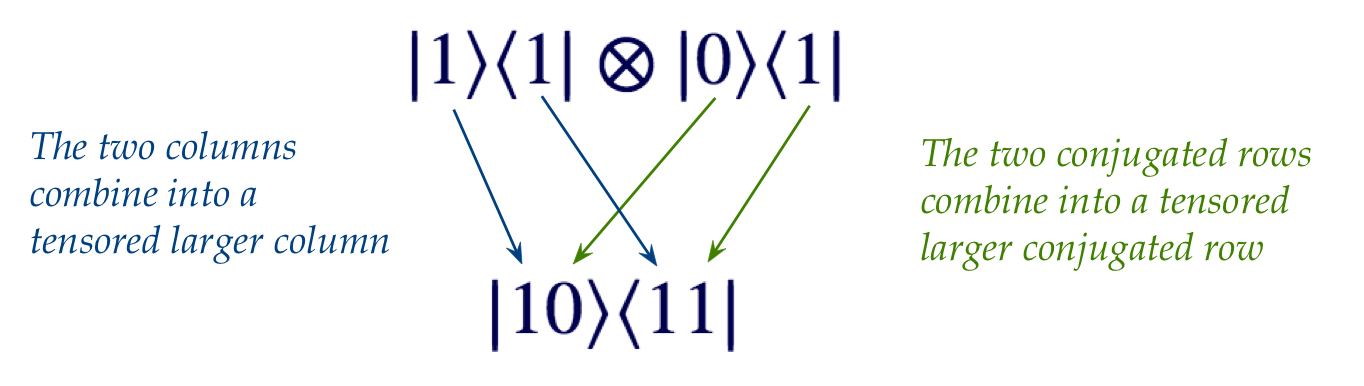
\includegraphics[width=4in]{notes/figs/n06/07tensor3.png}
        \caption{Column and conjugated row}
        \label{fig:06tensor1}
    \end{figure}
    
    Let's start familiarizing ourselves with some important unitary operators that form the foundation for building quantum computing circuits. First, let's look at the outer-product form for single qubit operators: We'll start with the simplest operator, the identity: Of course, we're used to writing
    
    $$
    I=\left[\begin{array}{ll}
    1 & 0 \\
    0 & 1
    \end{array}\right]
    $$
    
    But it can also be written in outer-product form as:
    
    $$
    I=|0\rangle\langle 0|+| 1\rangle\langle 1|
    $$
    
    because
    
    $$
    |0\rangle\langle 0|+| 1\rangle\langle 1|=\left[\begin{array}{ll}
    1 & 0
    \end{array}\right]\left[\begin{array}{l}
    1 \\
    0
    \end{array}\right]+\left[\begin{array}{ll}
    0 & 1
    \end{array}\right]\left[\begin{array}{l}
    0 \\
    1
    \end{array}\right]=\left[\begin{array}{ll}
    1 & 0 \\
    0 & 0
    \end{array}\right]+\left[\begin{array}{ll}
    0 & 0 \\
    0 & 1
    \end{array}\right]=\left[\begin{array}{ll}
    1 & 0 \\
    0 & 1
    \end{array}\right]
    $$
    
    We've seen that the "flip" operator $X$ can be written as
    
    $$
    X=|0\rangle\langle 1|+| 1\rangle\langle 0|=\left[\begin{array}{ll}
    0 & 1 \\
    0 & 0
    \end{array}\right]+\left[\begin{array}{ll}
    0 & 0 \\
    1 & 0
    \end{array}\right]=\left[\begin{array}{ll}
    0 & 1 \\
    1 & 0
    \end{array}\right]
    $$
    
    Note: An outer-product is written in terms of vectors $\triangleright$ It's an outer-product of vectors. The vectors used are orthonormal basis vectors. This way, algebraic expressions simplify through inner-products of basis vectors. Typically, we use the standard basis vectors, in the examples here. The advantage of using the outer-product form is that expressions can be simplified without expansion into a full-blown matrix. Example: let's see how this works with $X$ :
    
    $$
    \begin{aligned}
    X|0\rangle &=(|0\rangle\langle 1|+| 1\rangle\langle 0|)|0\rangle & & \text { Substitute outer prodact form } \\
    &=|0\rangle\langle 1|| 0\rangle+|1\rangle\langle 0|| 0\rangle & & \text { Distribution } \\
    &=|0\rangle(\langle 1 \mid 0\rangle)+|1\rangle(\langle 0 \mid 0\rangle) & & \text { Associativity } \\
    &=|1\rangle & & \text { Exploit orthonormal inner products }
    \end{aligned}
    $$
    
    The outer-product form is designed to exploit the simplifications obtained from pairing orthonormal basis vectors in inner products. Example:
    
    $$
    \begin{array}{rlr}
    X(\alpha|0\rangle+\beta|1\rangle) & =(|0\rangle\langle 1|+| 1\rangle\langle 0|)(\alpha|0\rangle+\beta|1\rangle) \quad \text { Look for cases where inner-product }=1 \\
    & =|0\rangle(\beta\langle 1 \mid 1\rangle)+|1\rangle(\alpha\langle 0 \mid 0\rangle) & \text { The ocher two are } 0 \text { from orthogonality } \\
    & =\beta|0\rangle+\alpha|1\rangle
    \end{array}
    $$
    
    The four Pauli operators:
    
    $$
    \begin{aligned}
    I=|0\rangle\langle 0|+| 1\rangle\langle 1| &=\left[\begin{array}{ll}
    1 & 0 \\
    0 & 1
    \end{array}\right] \\
    X=|0\rangle\langle 1|+| 1\rangle\langle 0| &=\left[\begin{array}{ll}
    0 & 1 \\
    1 & 0
    \end{array}\right] \\
    Y=-i|0\rangle\langle 1|+i| 1\rangle\langle 0| &=\left[\begin{array}{cc}
    0 & -i \\
    i & 0
    \end{array}\right] \\
    Z=|0\rangle\langle 0|-| 1\rangle\langle 1| &=\left[\begin{array}{cc}
    1 & 0 \\
    0 & -1
    \end{array}\right]
    \end{aligned}
    $$
    
    These are useful in quantum computing, and essential to quantum mechanics. Note: in quantum computing, the $Y$ operator is sometimes simplified to
    
    $$
    Y=-|1\rangle\langle 0|+| 0\rangle\langle 1|=\left[\begin{array}{cc}
    0 & 1 \\
    -1 & 0
    \end{array}\right]
    $$
    
    The $\mathrm{Z}$ operator results in change of relative phase:
    
    $$
    \begin{aligned}
    Z &=(|0\rangle\langle 0|-| 1\rangle\langle 1|)(\alpha|0\rangle+\beta|1\rangle) \\
    &=\alpha|0\rangle-\beta|1\rangle \\
    &=\alpha|0\rangle+e^{i \pi} \beta|1\rangle
    \end{aligned}
    $$
    
    Note: Recall that a unit-magnitude constant multiplying into a qubit state does not change the state, as in $e^{i \theta}(\alpha|0\rangle+\beta|1\rangle) \quad$ is the same state as $\quad \alpha|0\rangle+\beta|1\rangle$ But
    $e^{i \theta} \alpha|0\rangle+\beta|1\rangle \quad$ is different from $\quad \alpha|0\rangle+\beta|1\rangle$ and different from $\alpha|0\rangle+e^{i \theta} \beta|1\rangle$. Sometimes the notation
    
    $$
    \sigma_{1}=I \quad \sigma_{X}=X \quad \sigma_{Y}=Y \quad \sigma_{Z}=Z
    $$
    
    is used. Properties: The Pauli operators are both Hermitian and unitary. $X^{2}=Y^{2}=Z^{2}=I$. (Repeating returns a qubit to its original state.) Wolfgang Pauli was one of the first generation key contributors to the theory of quantum mechanics. (The others: Planck, Einstein, Heisenberg, Schrodinger, Born, Dirac, Bohr.) The Hadamard operator $H$ : $H$ is one of the most important operators in quantum computing. In both forms:
    
    $$
    H=\frac{1}{\sqrt{2}}(|0\rangle\langle 0|+| 1\rangle\langle 0|+| 0\rangle\langle 1|-| 1\rangle\langle 1|)=\frac{1}{\sqrt{2}}\left[\begin{array}{cc}
    1 & 1 \\
    1 & -1
    \end{array}\right]=\left[\begin{array}{cc}
    \frac{1}{\sqrt{2}} & \frac{1}{\sqrt{2}} \\
    \frac{1}{\sqrt{2}} & -\frac{1}{\sqrt{2}}
    \end{array}\right]
    $$
    
    Again, we can see how the outer-product simplifies application:
    
    $$
    \left.H|0\rangle \frac{1}{\sqrt{2}}(|0\rangle\langle 0|+| 1\rangle\langle 0|+| 0\rangle\langle 1|-| 1\rangle\langle 1|)|0\rangle=\frac{1}{\sqrt{2}}(|0\rangle+|1\rangle)=1+\right\rangle
    $$
    
    A relationship between $H$ and the Pauli operators:
    
    $$
    \begin{aligned}
    H &=\frac{1}{\sqrt{2}}(|0\rangle\langle 0|+| 1\rangle\langle 0|+| 0\rangle\langle 1|-| 1\rangle\langle 1|) \\
    &=\frac{1}{\sqrt{2}}((|0\rangle\langle 1|+| 1\rangle\langle 0|)+(|0\rangle\langle 0|-| 1\rangle\langle 1|)) \\
    &=\frac{1}{\sqrt{2}}(X+Z)
    \end{aligned}
    $$
    
    The outer-product form for 2 -qubit operators: A 2-qubit operator in matrix form is a $4 \times 4$ matrix. Any outer-product of two standard basis vectors gives us a matrix with a single 1 , the rest 0 's: Any outer-product of a basis vector with itself gives a 1 on the diagonal. Example:
    
    $$
    |10\rangle\langle 10|=\left[\begin{array}{l}
    0 \\
    0 \\
    1 \\
    0
    \end{array}\right]\left[\begin{array}{llll}
    0 & 0 & 1 & 0
    \end{array}\right]=\left[\begin{array}{llll}
    0 & 0 & 0 & 0 \\
    0 & 0 & 0 & 0 \\
    0 & 0 & 1 & 0 \\
    0 & 0 & 0 & 0
    \end{array}\right]
    $$
    
    A matrix with 1 in an off-diagonal location (0's elsewhere) can also be written as an outer-product. Example:
    
    $$
    \left[\begin{array}{llll}
    0 & 0 & 0 & 0 \\
    0 & 0 & 0 & 0 \\
    0 & 0 & 0 & 1 \\
    0 & 0 & 0 & 0
    \end{array}\right]=\left[\begin{array}{l}
    0 \\
    0 \\
    1 \\
    0
    \end{array}\right]\left[\begin{array}{llll}
    0 & 0 & 0 & 1
    \end{array}\right]=|10\rangle\langle 11|
    $$
    
    Then, any $4 \times 4$ matrix with 0 's and 1's can be written as a sum of such outer-products. Example:
    
    $$
    I=|00\rangle\langle 00|+| 01\rangle\langle 01|+| 10\rangle\langle 10|+| 11\rangle\langle 11|
    $$
    
    The $C_{N O \tau}$ operator: This is a 2-qubit operator. The matrix version:
    
    $$
    C_{\text {NOT }}=\left[\begin{array}{llll}
    1 & 0 & 0 & 0 \\
    0 & 1 & 0 & 0 \\
    0 & 0 & 0 & 1 \\
    0 & 0 & 1 & 0
    \end{array}\right]
    $$
    
    The outer-product form:
    
    $$
    C_{N o r}=|00\rangle\langle 00|+| 01\rangle\langle 01|+| 10\rangle\langle 11|+| 11\rangle\langle 10|
    $$
    
    One also frequently writes
    
    $$
    C_{N O T}=(|0\rangle\langle 0| \otimes I)+(|1\rangle\langle 1| \otimes X)
    $$
    
    It's not an exaggeration to say that $C_{N o r}$ is one of the most important operators in quantum computing. In fact, one basic test of any quantum hardware is whether it can perform $C_{N o r}$ reliably and quickly. Later, we will see that a few single-qubit operators and $C_{N O T}$ are sufficient to build larger arbitrary unitary operators. Proposition 4.13:
    $C_{\text {Nor }}$ cannot be expressed as a simple tensor of two 1-qubit operators. That is, no unitary operators $U_{1}, U_{2}$ exist such that $C_{N O T}=U_{1} \otimes U_{2}$. Proof: See solved problems. The implication: There are some operators that necessarily must be applied to 2 -qubits simultaneously. This is challenging to achieve in hardware but is necessary. Fortunately, as we'll see, this is sufficient in that larger multi-qubit operators can be constructed out of $C_{\text {Nor }}$ 's and 1-qubit operators.

\subsection{A few special bases}

    A few bases tend to get used more often than others in quantum computing: 1. The standard basis (single and multiple qubits) 2. The Hadamard basis (single and multiple qubits) 3. The Bell basis (two qubits). When does a basis matter? There are three cases when the choice of basis matters. First, and most importantly: when measurement occurs, the measuring device always has an associated basis. Thus, for example, if one measures in the Hadamard basis: The single-qubit Hadamard basis has: $|+\rangle,|-\rangle$. Then, a qubit state is expressed in this basis:
    
    $$
    \psi=\alpha|+\rangle+\beta|-\rangle
    $$
    
    After which, we know that an actual measurement will result in: $\begin{array}{ll}|+\rangle & \text { with probability }|\alpha|^{2} \\ |-\rangle & \text { with probability }|\beta|^{2}\end{array}$. If we measured in Hadamard but expressed in standard, we'd have to convert to Hadamard to assess probabilities, for example: Suppose
    
    $$
    |\psi\rangle=\frac{\sqrt{2}}{\sqrt{3}}|0\rangle+\frac{1}{\sqrt{3}}|1\rangle
    $$
    
    Converting to Hadamard, we see that
    
    $$
    |\psi\rangle=\frac{\sqrt{2}+1}{\sqrt{6}}|+\rangle+\frac{\sqrt{2}-1}{\sqrt{6}}|-\rangle
    $$
    
    Thus, the probabilities associated with measurement outcomes are:
    
    $$
    \begin{aligned}
    &\text { Observe }|+\rangle \quad \text { with probability }\left|\frac{\sqrt{2}+1}{\sqrt{6}}\right|^{2} \\
    &\text { Observe }|-\rangle \quad \text { with probability }\left|\frac{\sqrt{2}-1}{\sqrt{6}}\right|^{2}
    \end{aligned}
    $$
    
    The second case is when one is analyzing a Hermitian: Recall: a Hermitian packages projectors. And a tensored Hermitian does this across multiple qubits. Analysis is always easier when a Hermitian is expressed in the coordinates of its eigenvector basis. In this case, the Hermitian is a diagonal matrix (eigenvalues on the diagonal). We don't see much of this analysis in quantum computing but it's heavily used in quantum mechanics. The third instance where a basis matters is when the vectors in the basis serve a special purpose. This is the case with the Bell basis, as we'll see. The standard basis. For a single qubit, the standard basis is: $|0\rangle \quad|1\rangle$. For two qubits: $|00\rangle, \quad|01\rangle, \quad|10\rangle, \quad|11\rangle$. For $\mathrm{n}$-qubits, it's the $2^{n}$ vectors
    
    $$
    |00 \ldots 0\rangle, \quad|00 \ldots 1\rangle, \quad \ldots \quad|11 \ldots 1\rangle
    $$
    
    The standard basis is the most commonly used basis in quantum computing: Most states are expressed in this basis. And most measurements occur in this basis. Decimal shorthand notation: The binary strings are interpreted as decimal numbers. Thus, the 2-qubit basis is also written as: $|0\rangle,|1\rangle,|2\rangle,|3\rangle$. The n-qubit: $|0\rangle,|1\rangle, \ldots,\left|2^{n}-1\right\rangle$. Thus, the 3 -qubit basis is written in these two ways:
    
    \begin{align*}
        |0\rangle & =|000\rangle\\
        |1\rangle & =|001\rangle\\
        |2\rangle & =|010\rangle\\
        |3\rangle & =|011\rangle\\
        |4\rangle & =|100\rangle\\
        |5\rangle & =|101\rangle\\
        |6\rangle & =|110\rangle\\
        |7\rangle & =|111\rangle
    \end{align*}

    The Hadamard basis: This is typically used in the single-qubit case for measurement. The two basis vectors: $|+\rangle,|-\rangle$. These vectors themselves can of course be expressed in the standard basis:
    
    $$
    \begin{aligned}
    |+\rangle &=\frac{1}{\sqrt{2}}(|0\rangle+|1\rangle) \\
    |-\rangle &=\frac{1}{\sqrt{2}}(|0\rangle-|1\rangle)
    \end{aligned}
    $$
    
    We saw one example: polarization. And we saw its use in the BB- $84 \mathrm{key}$-distribution protocol. The Hadamard unitary operator, on the other hand, is often used in the multiple-qubit case where it is tensored. The Bell basis: This is a 2 -qubit basis with the following four vectors:
    
    $$
    \begin{aligned}
    \left|\Phi^{+}\right\rangle &=\frac{1}{\sqrt{2}}(|00\rangle+|11\rangle) \\
    \left|\Phi^{-}\right\rangle &=\frac{1}{\sqrt{2}}(|00\rangle-|11\rangle) \\
    \left|\Psi^{+}\right\rangle &=\frac{1}{\sqrt{2}}(|01\rangle+|10\rangle) \\
    \left|\Psi^{-}\right\rangle &=\frac{1}{\sqrt{2}}(|01\rangle-|10\rangle)
    \end{aligned}
    $$
    
    Sometimes these are also named $\beta_{00}, \beta_{01}, \beta_{10}, \beta_{11}$. (Well use the former.) This basis is not really used for measurement but instead, one or more of these vectors are used as a desirable state to initiate a computation, as well see below.

\subsection{Entanglement: a first look}

    Consider the first Bell vector:
    
    $$
    \left|\Phi^{+}\right\rangle=\frac{1}{\sqrt{2}}(|00\rangle+|11\rangle)
    $$
    
    This is a 2-qubit state. Let's ask: are there two 1-qubit states $|v\rangle$ and $|w\rangle$ such that
    
    $$
    \left|\Phi^{+}\right\rangle=|v\rangle \otimes|w\rangle ?
    $$
    
    Let
    
    $$
    \begin{aligned}
    |v\rangle &=\alpha_{0}|0\rangle+\alpha_{1}|1\rangle \\
    |w\rangle &=\beta_{0}|0\rangle+\beta_{1}|1\rangle
    \end{aligned}
    $$
    
    Then,
    
    $$
    \begin{aligned}
    |v\rangle \otimes|w\rangle &=\left(\alpha_{0}|0\rangle+\alpha_{1}|1\rangle\right) \otimes\left(\beta_{0}|0\rangle+\beta_{1}|1\rangle\right) \\
    &=\alpha_{0} \beta_{0}(|0\rangle \otimes|0\rangle)+\alpha_{0} \beta_{1}(|0\rangle \otimes|1\rangle)+\alpha_{1} \beta_{0}(|1\rangle \otimes|0\rangle)+\alpha_{1} \beta_{1}(|1\rangle \otimes|1\rangle) \\
    &=\alpha_{0} \beta_{0}|00\rangle+\alpha_{0} \beta_{1}|01\rangle+\alpha_{1} \beta_{0}|10\rangle+\alpha_{1} \beta_{1}|11\rangle
    \end{aligned}
    $$
    
    Now equate this to $\left|\Phi^{+}\right\rangle$:
    
    $$
    \alpha_{0} \beta_{0}|00\rangle+\alpha_{0} \beta_{1}|01\rangle+\alpha_{1} \beta_{0}|10\rangle+\alpha_{1} \beta_{1}|11\rangle=\frac{1}{\sqrt{2}}(|00\rangle+|11\rangle)
    $$
    
    Notice that the existence of $|00\rangle$ implies $\alpha_{0}$ and $\beta_{0}$ are both nonzero. Similarly |11) implies $\alpha_{1}$ and $\beta_{1}$ are both nonzero. This would force inclusion of $|01\rangle$ and $|10\rangle$ on the left. Thus, no tensoring of 1-qubit vectors can equal $\left|\Phi^{+}\right\rangle$. Yet $\left|\Phi^{+}\right\rangle$is a valid 2-qubit state because it's a linear combination of 2 -qubit basis vectors:
    
    $$
    \left|\Phi^{+}\right\rangle=\frac{1}{\sqrt{2}}|00\rangle+\frac{1}{\sqrt{2}}|11\rangle
    $$
    
    What we've discovered is this: Let $B_{1}$ be the basis vectors $|0\rangle,|1\rangle$ for the first qubit, and $V_{1}$ be the vector space
    
    $$
    V_{1}=\left\{\alpha_{0}|0\rangle+\alpha_{1}|1\rangle\right\}
    $$
    
    That is, unit-length linear combinations of the basis vectors of space $V_{1}$. Let $B_{2}$ and $V_{2}$ be the corresponding basis, and vector space for the 2 nd qubit:
    
    $$
    V_{2}=\left\{\beta_{0}|0\rangle+\beta_{1}|1\rangle\right\}
    $$
    
    We construct the 2-qubit vector space by first putting together its basis $B_{1,2}$ by tensoring the basis vectors from $V_{1}$ and $V_{2}$ :
    
    $$
    B_{1,2}=\{|0\rangle \otimes|0\rangle,|0\rangle \otimes|1\rangle+|1\rangle \otimes|0\rangle,|1\rangle \otimes|1\rangle,\}=\{|00\rangle,|01\rangle,|10\rangle,|11\rangle\}
    $$
    
    Then, the vectors in the space $V_{1} \otimes V_{2}$ are linear combinations of these basis vectors:
    
    $$
    V_{1} \otimes V_{2}=\left\{a_{00}|00\rangle+a_{01}|01\rangle+a_{10}|10\rangle+a_{11}|11\rangle\right\}
    $$
    
    Now, there are vectors in $V_{1} \otimes V_{2}$ that can be expressed as tensors of smaller vectors, one each in $V_{1}$ and $V_{2}$, for example: Let $|0\rangle$ be an example vector from $V_{1}$ (1st qubit). Let
    
    $$
    \frac{\sqrt{2}}{\sqrt{3}}|0\rangle+\frac{1}{\sqrt{3}}|1\rangle
    $$
    
    be a vector from $V_{2}$. Now,
    
    $$
    |\psi\rangle=\frac{\sqrt{2}}{\sqrt{3}}|00\rangle+\frac{1}{\sqrt{3}}|01\rangle
    $$
    
    is a vector in $V_{1} \otimes V_{2}$ because it's a linear combination of basis vectors. And it's expressible as a tensor of the smaller vectors:
    
    $$
    \begin{aligned}
    |0\rangle \otimes\left(\frac{\sqrt{2}}{\sqrt{3}}|0\rangle+\frac{1}{\sqrt{3}}|1\rangle\right) &=\frac{\sqrt{2}}{\sqrt{3}}(|0\rangle \otimes|0\rangle)+\frac{1}{\sqrt{3}}(|0\rangle \otimes|1\rangle) \\
    &=\frac{\sqrt{2}}{\sqrt{3}}|00\rangle+\frac{1}{\sqrt{3}}|01\rangle \\
    &=|\psi\rangle
    \end{aligned}
    $$
    
    At the same time, there are vectors in $V_{1} \otimes V_{2}$ that cannot be expressed as tensored smaller vectors:
    
    $$
    \left|\Phi^{+}\right\rangle \neq\left|v_{1}\right\rangle \otimes\left|v_{2}\right\rangle
    $$
    
    for any $\left|v_{1}\right\rangle \in V_{1},\left|v_{2}\right\rangle \in V_{2}$. Definitions: A vector like $\left(\Phi^{+}\right\rangle$that cannot be expressed by tensoring smaller vectors is called an entangled vector. A vector like $|\psi\rangle$ that can be expressed as such is called a separable vector. The term entanglement refers both to: The phenomenon, as described above. Physical implementations where two qubits are deliberately set up so that the combined 2 -qubit state is entangled. More about entanglement: Entanglement is a property of how tensoring is set up. Once we have a tensor product defined, an entangled vector from the larger space is entangled no matter what bases are used. It is possible for a larger system to be constructed by tensoring subsystems in different ways. Then, it's possible for a larger-system state to be entangled with respect to one subsystem but not the other. (See the Rieffel book for an example.) In this course, the tensor products we will see won't have this issue. The most important (and weird) consequence of entanglement: Consider flying qubits. One can create a pair of such qubits in an entangled state as shown in Figure \ref{fig:08entangle1}.
    
    \begin{figure}
        \centering
        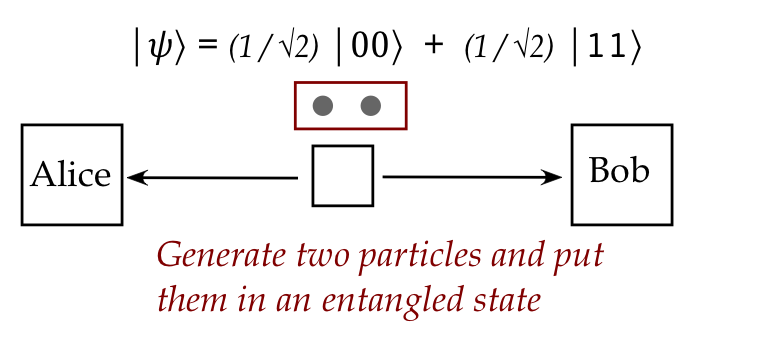
\includegraphics[width=4in]{notes/figs/n06/08entangle1.png}
        \caption{Two particles in an entangled state}
        \label{fig:08entangle1}
    \end{figure}
    
    Then, these qubits can be physically separated and sent in different directions as shown in Figure \ref{fig:09entangle2}.
    
    \begin{figure}
        \centering
        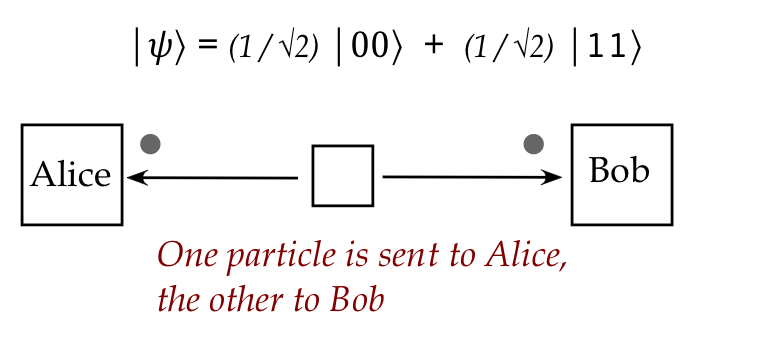
\includegraphics[width=4in]{notes/figs/n06/09entangle2.png}
        \caption{Physically separated}
        \label{fig:09entangle2}
    \end{figure}
    
    What's truly astonishing: The two particles maintain their entangled state no matter what the intervening distance. The implication is shown in Figure \ref{fig:10entangle3}.
    
    \begin{figure}
        \centering
        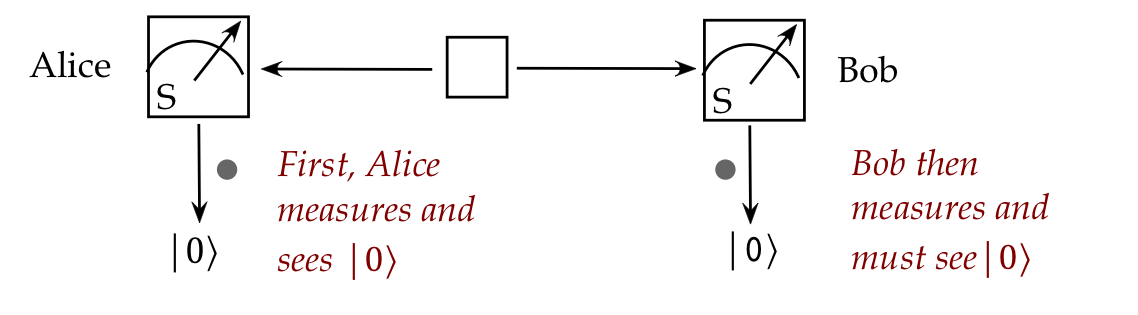
\includegraphics[width=4in]{notes/figs/n06/10entangle3.png}
        \caption{Entangled state}
        \label{fig:10entangle3}
    \end{figure}
    
    If Alice measures her qubit and sees $|0\rangle$, then Bob's single-qubit measurement performed afterwards will result in $|0\rangle !$ Note: At the time of measurement, Alice won't know which outcome, $|0\rangle$ or $|1\rangle$, will appear. But whichever outcome appears, Bob will see the same even if his measurement occurs much later. This is what Einstein termed "spooky action at a distance". We will later undertake a more careful analysis of how entangled particles might have this property: Instead of explaining away this property in a straightforward way, the analysis will only deepen the mystery. A pair of entangled particles is sometimes called an EPR pair, after Einstein-Podolsky-Rosen, whose 1935 paper first raised the possibility of entangled pairs and "spooky action" as a way to question whether quantum mechanics was complete.
    
\subsection{The E91 key distribution protocol: a first glimpse}

    Recall the goal of key distribution: Alice and Bob want to create a shared secret key for future communications. This secret key is a (classical) random binary string like $10100111010101101 \ldots$ (long enough, for high security). Then, future text messages use the same key to encrypt (on one side), and decrypt (on the other). The actual encryption mechanism can use the key in different ways. For example: apply XOR using the key to a binary text message. Recall from BB84: BB84 has Alice create and send qubits to Bob. After that, they apply measurements in different bases. Then, they compare basis-choices afterwards, and when in agreement, use the corresponding qubits. Note: Eve can intercept the qubits to try and attack. The E91 protocol is named after Artur Ekert, who published this idea in $1991$. What's interesting: No qubits are exchanged. Eve has nothing to work with! The E91 protocol: The protocol assumes that Alice and Bob share a number of entangled qubits as shown in Figure \ref{fig:11ekert2}.
    
    \begin{figure}
        \centering
        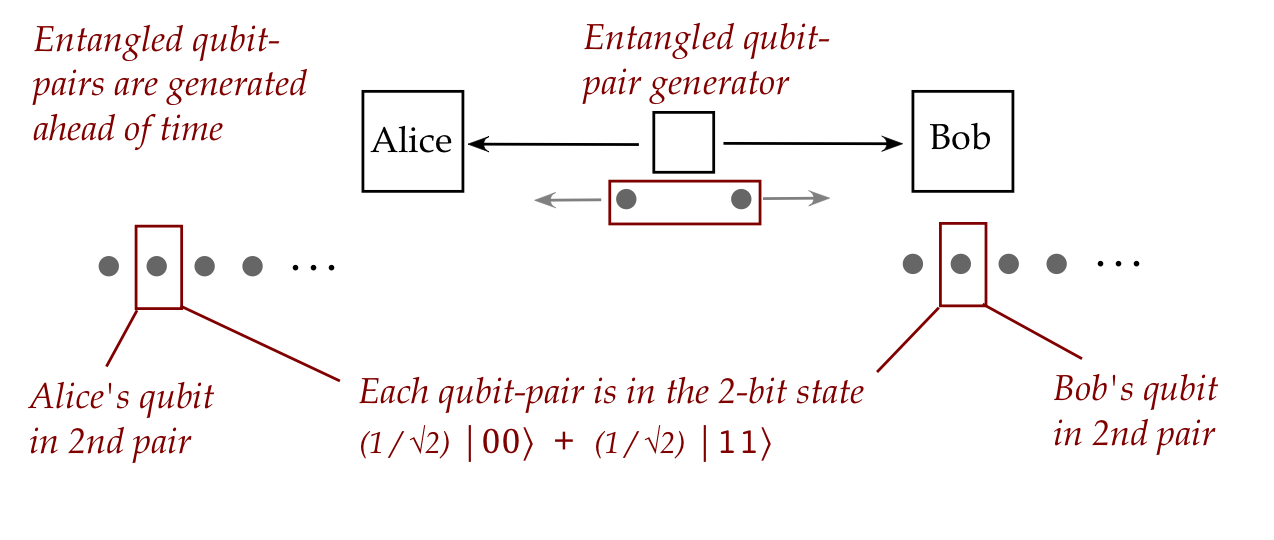
\includegraphics[width=4in]{notes/figs/n06/11ekert2.png}
        \caption{shared entangled qubits}
        \label{fig:11ekert2}
    \end{figure}
    
    $n$ entangled pairs are generated, each in the state
    
    $$
    \left|\Phi^{+}\right\rangle=\frac{1}{\sqrt{2}}(|00\rangle+|11\rangle)
    $$
    
    One qubit in each pair is sent to Alice. The other is sent to Bob. So, at the start, Alice and Bob each have $n$ qubits. At this stage, there is no key information exchanged. At the start of the protocol, Alice and Bob share a classical channel shown in Figure \ref{fig:12ekert1}.

    \begin{figure}
        \centering
        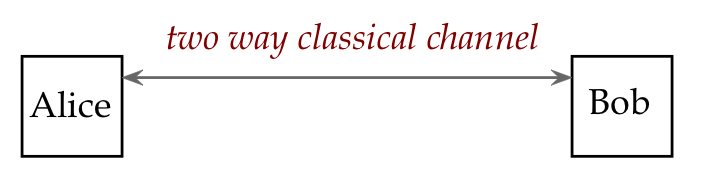
\includegraphics[width=4in]{notes/figs/n06/12ekert1.png}
        \caption{shared classical channel}
        \label{fig:12ekert1}
    \end{figure}
    
    Note: No qubits are transmitted during the protocol. Step 1: they each independently choose (without communication) an S-H string shown in Figure \ref{fig:13ekert3}.
    
    \begin{figure}
        \centering
        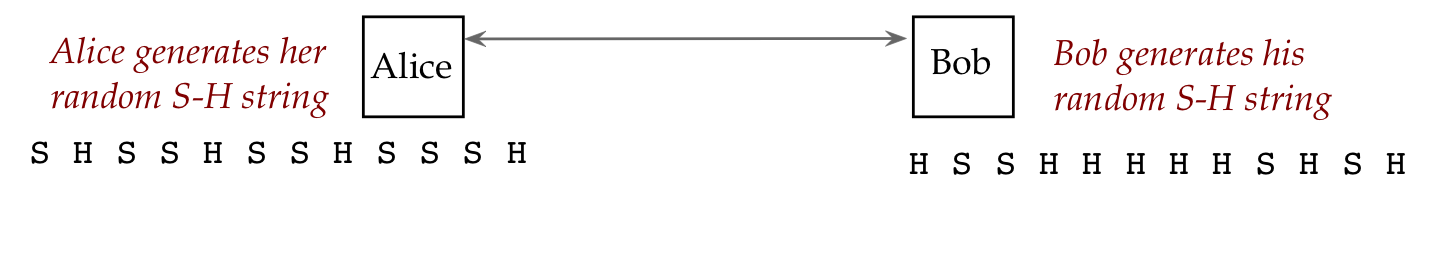
\includegraphics[width=4in]{notes/figs/n06/13ekert3.png}
        \caption{Independently choose S-H string}
        \label{fig:13ekert3}
    \end{figure}
    
    Note: the two S-H strings are expected to be non-identical. Again, no information exchanged thus far. Step 2: Alice measures her qubit of each pair as shown in Figure \ref{fig:14ekert4}.
    
    \begin{figure}
        \centering
        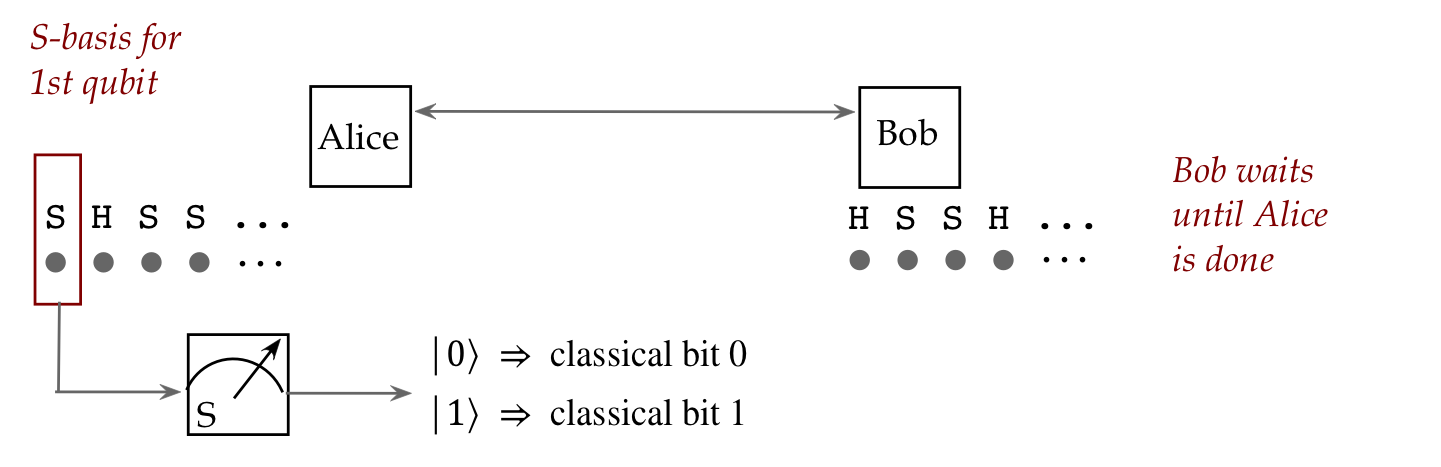
\includegraphics[width=4in]{notes/figs/n06/14ekert4.png}
        \caption{Alice measures}
        \label{fig:14ekert4}
    \end{figure}
    
    She measures in the S-basis, if the i-th letter is $\mathrm{S}$ in her $\mathrm{S}-\mathrm{H}$ string. Otherwise, she uses the H-basis. If she uses the S-basis, she produces a classical bit according to:
    
    $$
    \begin{array}{ll}
    \text { bit }=0 & \text { if outcome is }|0\rangle \\
    \text { bit }=1 & \text { if outcome is }|1\rangle
    \end{array}
    $$
    
    With the H-basis:
    
    $$
    \begin{array}{ll}
    \text { bit }=0 & \text { if outcome is }|+\rangle \\
    \text { bit }=1 & \text { if outcome is }|-\rangle
    \end{array}
    $$
    
    Step 3: Bob now measures his qubit of each pair shown in Figure \ref{fig:15ekert5}.
    
    \begin{figure}
        \centering
        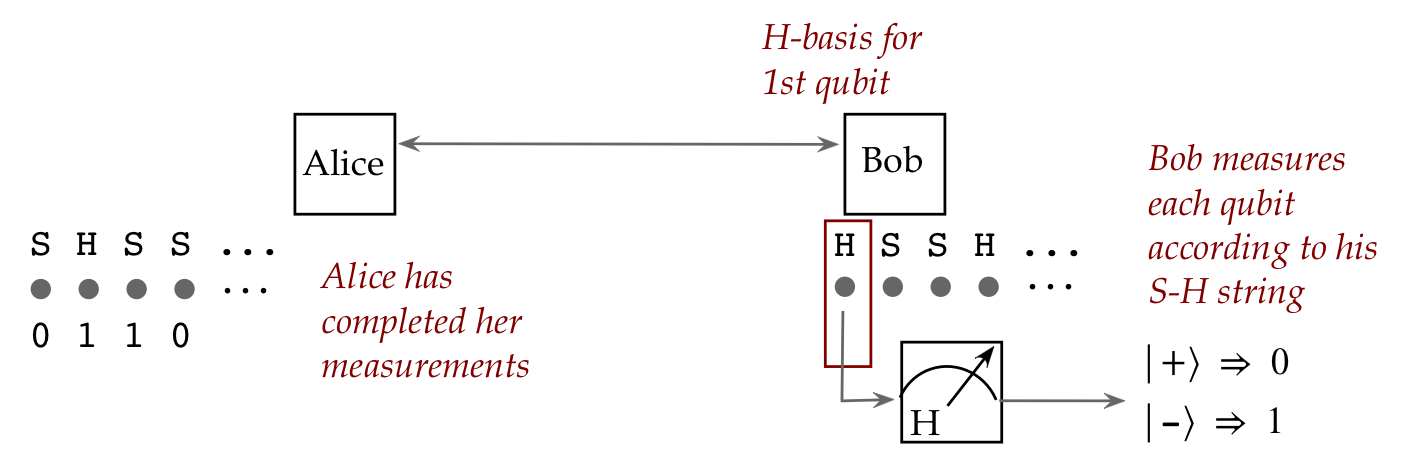
\includegraphics[width=4in]{notes/figs/n06/15ekert5.png}
        \caption{Bob measures}
        \label{fig:15ekert5}
    \end{figure}
    
    He applies the S-basis measurement, if the i-th letter is $\mathrm{S}$ in his $\mathrm{S}$-H string. Otherwise, he measures with the H-basis. He uses the same rule for mapping measurement outcomes to classical bits. Step 4: They now share their S-H strings through the classical channel shown in Figure \ref{fig:16ekert6}.
    
    \begin{figure}
        \centering
        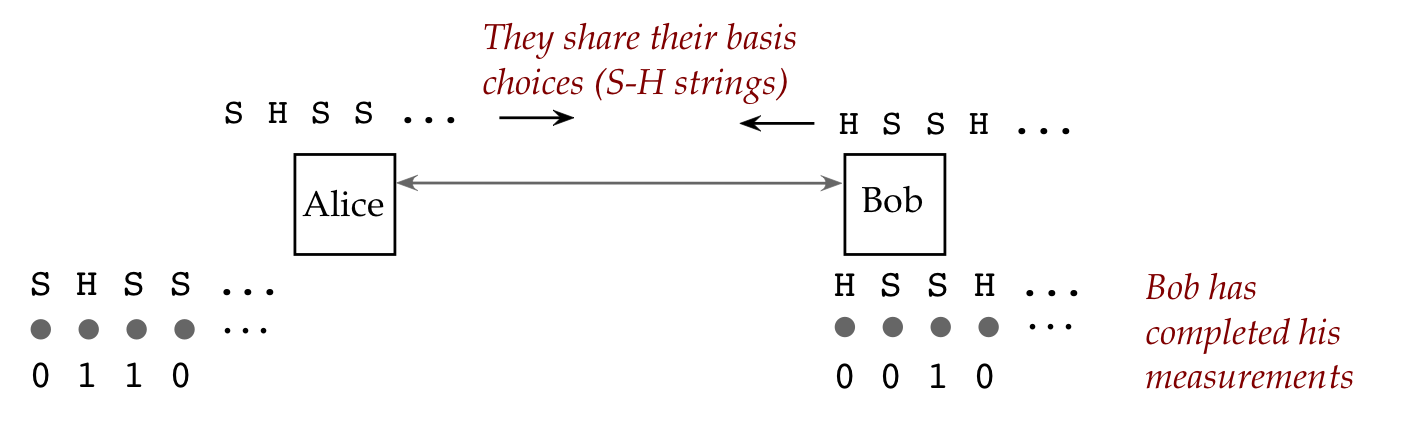
\includegraphics[width=4in]{notes/figs/n06/16ekert6.png}
        \caption{share basis choices}
        \label{fig:16ekert6}
    \end{figure}
    
    Step 5: They keep all the classical bits where their S-H string values matched shown in Figure \ref{fig:17ekert7}.
    
    \begin{figure}
        \centering
        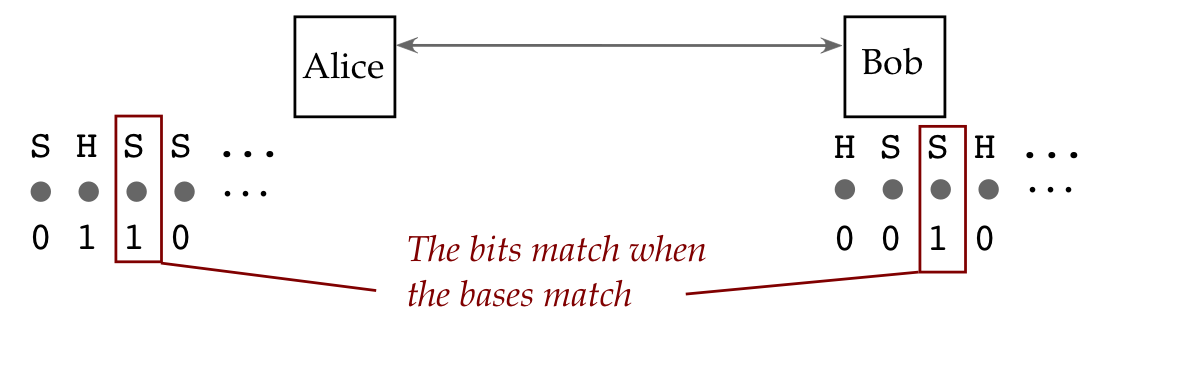
\includegraphics[width=4in]{notes/figs/n06/17ekert7.png}
        \caption{bits basis match}
        \label{fig:17ekert7}
    \end{figure}
    
    The i-th classical bit is kept when they used the same basis for the i-th qubit measurement. Otherwise, the classical bit is discarded. The result is a secret key. The protocol relies on what happens with measurement with an entangled pair: Let's focus on the cases where their bases match. Consider when Alice measures with S-basis: Suppose the outcome is $|0\rangle$. Then, Bob's outcome is also $|0\rangle$ (with certainty). This is easy to see with the entangled state:
    
    $$
    \left|\Phi^{+}\right\rangle=\frac{1}{\sqrt{2}}(|00\rangle+|11\rangle)
    $$
    
    If Alice sees $|0\rangle$, the combined 2-qubit state is:
    
    $$
    |00\rangle=|0\rangle \otimes|0\rangle
    $$
    
    which means Bob's qubit must be measured as $|0\rangle$. We can summarize this as: when both use the S-basis in sequence, both interpretations match as shown in Figure \ref{fig:18ekert8}.
    
    \begin{figure}
        \centering
        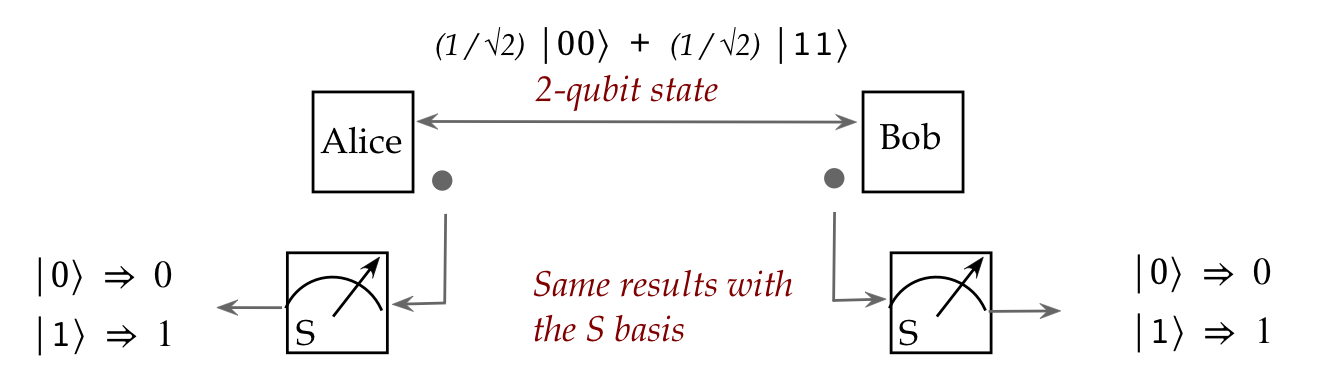
\includegraphics[width=4in]{notes/figs/n06/18ekert8.png}
        \caption{S-basis interpretations match}
        \label{fig:18ekert8}
    \end{figure}    
    
    What is less clear at the moment is that the same holds with the H-basis \ref{fig:19ekert9},
    
    \begin{figure}
        \centering
        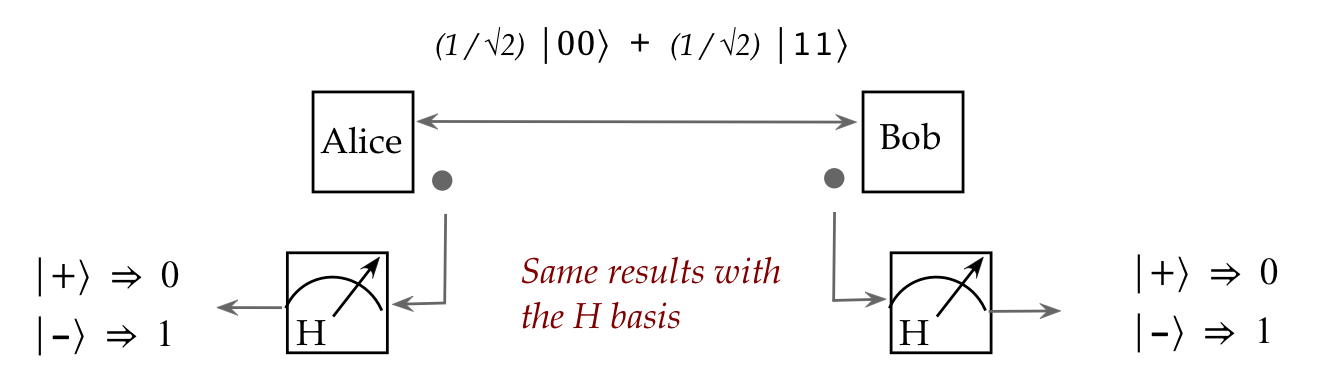
\includegraphics[width=4in]{notes/figs/n06/19ekert9.png}
        \caption{H-basis results}
        \label{fig:19ekert9}
    \end{figure} 
    
    When Alice uses the H-basis and sees $|+\rangle$ the outcome state is:
    
    $$
    |+\rangle \otimes|+\rangle
    $$
    
    Thus, Bob's H-basis measurement leads to the same outcome. When we learn about how 2 -qubit measurement works, we'll re-examine this part. What can Eve do? We assume that the classical channel is secure (perhaps using a previously generated key). Alice and Bob do not communicate qubits. There is nothing for Eve to intercept. However, Eve could have tampered with the earlier generation of entangled pairs. As in BB84, Alice and Bob can sacrifice some key bits to test whether the pairs are properly entangled. They perform measurements to see if the results match what entanglement predicts. Practicalities: The really hard part, in practice, is storing entangled qubits. There is active on-going research in photon storage. Other approaches seek to entangle a flying qubit with a stationary qubit, so that stationary qubits can maintain entangled state.

\subsection{Aside: Commutators, direct sums}

    We will occasionally use these asides to point out terminology and concepts that are related but not directly required for quantum computing. About commutators: We know that matrix multiplication is not commutative, i.e., in general
    
    $$
    A B \neq B A
    $$
    
    One useful quantification of "how non-commutative" for two operators $A$ and $B$ is the so-called commutator
    
    $$
    [A, B] \triangleq A B-B A
    $$
    
    Then, clearly, A commutes with $B$ if $[A, B]=0$. One powerful result is that if $[A, B]=0$, one can find a common eigenbasis for both $A$ and $B$. In this case, when $A$ and $B$ are measurement operators, the outcomes of measurement are the same. Then, measurement with $A$ produces predictable outcomes with $B$. Thus, Heisenberg uncertainty is not present (or zero) for commuting measurement operators. When $[A, B] \neq 0$ Heisenberg's uncertainty principle can be quantified in terms of a lower bound featuring the commutator $[A, B]$. Direct sums: Just as the tensor product $\otimes$ is a "sort of" product, one could ask: is there an equivalent "sort of" sum? The answer: yes. Well provide only a quick and dirty intuitive overview. Consider the two vectors
    
    $$
    |v\rangle=\left[\begin{array}{l}
    1 \\
    2 \\
    3
    \end{array}\right] \quad|w\rangle=\left[\begin{array}{l}
    4 \\
    5
    \end{array}\right]
    $$
    
    Clearly, they are incompatible for regular addition, coming from different vector spaces. However, one can expand both into
    
    $$
    |v\rangle=\left[\begin{array}{l}
    1 \\
    2 \\
    3 \\
    0 \\
    0
    \end{array}\right] \quad|w\rangle=\left[\begin{array}{l}
    0 \\
    0 \\
    0 \\
    4 \\
    5
    \end{array}\right]
    $$
    
    They are now addition-compatible
    
    $$
    |v\rangle \oplus|w\rangle=\left[\begin{array}{l}
    1 \\
    2 \\
    3 \\
    4 \\
    5
    \end{array}\right]
    $$
    
    In this manner, one can construct the direct sum of two differently-dimensioned vector spaces $V$ and $W$ : Suppose $V$ has basis vectors $\left|v_{1}\right\rangle, \ldots,\left|v_{m}\right\rangle$. Any vector $v \in V$ has $m$ elements. Suppose $W$ has basis vectors $\left|w_{1}\right\rangle, \ldots,\left|w_{n}\right\rangle$. Any vector $w \in W$ has $n$ elements. We add trailing $n$ trailing 0 's to every $v \in V$. And prefix $m 0$ 's to every $w \in W$. Now all vectors have $m+n$ elements. Then, a basis for the direct sum space $V \oplus W$ are the $m+n$ vectors.
    
    $$
    \left|v_{1}\right\rangle, \ldots,\left|v_{m}\right\rangle,\left|w_{1}\right\rangle, \ldots,\left|w_{n}\right\rangle
    $$
    
    Where is this useful? Notice that orthonormal subspaces "direct sum" into the original space. For example, with real vectors, let.
    
    $$
    \begin{aligned}
    V &=\text { all vectors in the } \mathrm{x} \text {-y plane } \\
    W &=\text { all vectors along } \mathrm{z} \text {-axis }
    \end{aligned}
    $$
    
    Then $V \oplus W$ is 3D space. When we look further into projective measurement, what we'll see is that measurement outcomes divide into such direct-sum subspaces. Thus, the usefulness comes in providing a rigorous mathematical foundation to measurement.

\subsection{Matrix exponentials and fractional powers}

    Recall how we defined the exponential of a complex number: The rules of addition and multiplication for real numbers were extended to complex numbers in a straightforward way. (See Module 2.). But it's not obvious how one exponentiates a complex number $z$ to calculate $e^{z}$. The way forward came about by looking at the Taylor series expansion for the real function $e^{x}$
    
    $$
    e^{x}=1+x+\frac{x^{2}}{2 !}+\frac{x^{3}}{3 !}+\ldots
    $$
    
    The right side has only arithmetic operations. From this, we defined the complex exponential
    
    $$
    e^{z} \triangleq 1+z+\frac{z^{2}}{2 !}+\frac{z^{3}}{3 !}+\ldots
    $$
    
    which eventually led to Euler's relation:
    
    $$
    e^{i \theta}=\cos \theta+i \sin \theta
    $$
    
    The same approach can be used to define matrix exponentiation: First, let's ask: what arithmetic operations do we already have with matrices? Answer: We have addition $A+B$ for matrices $A, B$. We have multiplication $A B$. Scalar multiplication $\alpha A$. From this follows powers of a matrix:
    
    $$
    A^{k}=A A \ldots A \quad \text { (multiplication } k \text { times) }
    $$
    
    Then, for a matrix $A$, define
    
    $$
    e^{A} \triangleq I+A+\frac{A^{2}}{2 !}+\frac{A^{3}}{3 !}+\ldots
    $$
    
    The right side uses operations that already exist and so, if the infinite series converges, we have a working definition. It can be shown (not easily) that the infinite series does converge for complex-valued matrices. Two forms of the matrix exponential are commonly used: The direct form, as above. With an additional scalar variable
    
    $$
    e^{\alpha A} \triangleq I+\alpha A+\frac{\alpha^{2} A^{2}}{2 !}+\frac{\alpha^{3} A^{3}}{3 !}+\ldots
    $$
    
    When the scalar is $\alpha=i$, we get the complex matrix exponential $e^{i A}$. This is useful in quantum computing because, if $A$ is Hermitian, then $e^{i A}$ is unitary because
    
    $$
    \left(e^{i A}\right)^{\dagger} e^{i A}=e^{-i A A^{\dagger}} e^{i A}=e^{-i A} e^{i A}=I
    $$
    
    (Note: it's true but far from obvious that $\left(e^{i A}\right)^{\dagger}=e^{-i A^{\prime}}$.) In particular, the four Pauli operators $I, X, Y, Z$ are Hermitian: Then, $e^{i I}, e^{i X}, e^{i Y}, e^{i Z}$ are all unitary matrices. Some of these are useful in practice. We'll merely list a bunch of properties without proof: If $D$ is a (square) diagonal matrix with diagonal entries $d_{1}, \ldots, d_{n}$, then
    
    $$
    e^{D}=\left[\begin{array}{cccc}
    e^{d_{1}} & 0 & 0 & 0 \\
    0 & e^{d_{2}} & 0 & 0 \\
    0 & 0 & \ddots & 0 \\
    0 & 0 & 0 & e^{d_{n}}
    \end{array}\right]
    $$
    
    If $A$ can be written as $A=S D S^{-1}$ where $D$ is diagonal and $S$ is some matrix with an inverse, then
    
    $$
    e^{S D S^{-1}}=S e^{D} S^{-1}
    $$
    
    $\left(e^{A}\right)^{T}=e^{A^{T}}$, $e^{\left(z_{1}+z_{2}\right) A}=e^{z_{1} A}+e^{z_{2} A}$ for complex numbers $z_{1}, z_{2}$ , If $A B=B A$ then $e^{A} e^{B}=e^{A+B}$. A result that will be useful in quantum computing: $\circ$ If $A^{2}=I$ then
    
    $$
    \begin{aligned}
    e^{i \theta A} &=I+(i \theta) A+(i \theta)^{2} \frac{A^{2}}{2 !}+(i \theta)^{3} \frac{A^{3}}{3 !}+\ldots \\
    &=\left(I-\theta^{2} A^{2}+\theta^{4} A^{4} \ldots\right)+\left(i \theta A-i^{3} \theta^{3} A^{3}+i^{5} \theta^{5} A^{5} \ldots\right) \\
    &=\left(I-\theta^{2} I+\theta^{4} I \ldots\right)+\left(i \theta A-i \theta^{3} A^{2} A+i \theta^{5} A^{4} A \ldots\right) \\
    &=\left(1-\theta^{2}+\theta^{4} \ldots\right) I+\left(\theta-\theta^{3}+\theta^{5} \ldots\right) i A \\
    &=I \cos \theta+i A \sin \theta
    \end{aligned}
    $$
    
    Fractional powers: We know how positive integral powers like $A^{k}$ work. But what about $A^{\frac{1}{2}}$ or $A^{\frac{1}{\pi}}$ for integer $n$ ? The definition is easy: $X=A^{\frac{1}{n}}$ if $X^{n}=A$. But computing such fractional powers is complicated. And it isn't clear how many $\mathrm{n}$-th roots exist. For example,
    
    $$
    \left[\begin{array}{cc}
    a & b \\
    c & -a
    \end{array}\right]^{2}=\left[\begin{array}{cc}
    a^{2}+b c & 0 \\
    0 & a^{2}+b c
    \end{array}\right]
    $$
    
    Which means for any values of $a, b, c$ such that $a^{2}+b c=1$, the matrix
    
    $$
    \left[\begin{array}{cc}
    a & b \\
    c & -a
    \end{array}\right]=\left[\begin{array}{ll}
    1 & 0 \\
    0 & 1
    \end{array}\right]^{\frac{1}{2}}
    $$
    
    Thus, $I$ has an infinite number of square roots! If $A$ is Hermitian then it can be written as (Recall: the spectral theorem):
    
    $$
    A=S D S^{-1}
    $$
    
    Then
    
    $$
    \left(S D^{\frac{1}{2}} S^{-1}\right)^{2}=A
    $$
    
    Which means any combination of real-valued diagonal square roots elements of $D$ will be a square root of $A$. $A$ has $2^{n}$ square roots of the form $S D^{\frac{1}{2}} S^{-1}$

\subsection{Summary}

    Between this module and the earlier Module 2, we have covered a lot of new linear algebra: Complex numbers and vectors. The entirely new and somewhat strange Dirac notation. Unit-length simplification, phase equivalence. Important types of operators: projector, unitary, Hermitian. The sandwich. Tensors for vectors, tensors for operators. Some well-known bases. Entanglement, including an application of this strange phenomenon. Matrix exponentials and fractional powers. Fortunately, this is all the linear algebra we need. The Dirac notation does take acclimation, and that happens by doing the (occasionally tedious) exercises, and trying out the solved problems on your own.

\end{document}